%Contains the restructured agent design etc.

\chapter{Stochastic Target Localisation}\label{chap:targetLocalisation}
This chapter outlines the approach taken to address the first research question stated in the introduction chapter:
\\
"\textit{Can an agent-based software system be developed to run on a system of heterogeneous autonomous aerial vehicles to aid the tasks of scene surveying and target localisation in a hazardous environment? }"
\\
This Chapter deals specifically with the problem of \textit{target localisation}, which we explain in precise terms in Section \ref{sec:TLocalisationProbDescription}. The context for this problem is derived from the ROCSAFE project \cite{Bagherzadeh2017ROCSAFE:Incidents}. We first give the technical description of the problem and simplifying assumptions that we made. We then discuss the testbed that was used to prototype the solution. We used a DBN to model the agent's environment, described subsequently. Finally, we present the results of running monte carlo simulations to evaluate the system performance. We designed agents to perform the search, taking a similar approach to the recent literature, noted in Section \ref{sec:StochasticTargetLocalisationRelatedLiterature}.

\section{Problem Description}\label{sec:TLocalisationProbDescription}
As mentioned in Chapter \ref{chapter:introduction}, a major problem in hazardous scene management includes localizing sources of hazardous materials and localizing potential sources of evidence. The reasons these are difficult problems, in the context of the ROCSAFE project, are:
\begin{itemize}
    \item Hazardous materials belong to different classes of threat (chemical, biological, radiation, nuclear). If the nature of the threat is uncertain, the wrong preventative measures may be taken and personnel may be put at risk. 
    \item Evidence localisation usually requires moving a sensor to within close proximity of the evidence. If a human is responsible for this, there is a chance that they will accidentally disturb with the evidence, possibly yielding it unusable.
    \item Since these scenarios are highly dangerous, the area to search may be large to avoid potentially missing important sources of evidences. This means that the process of localisation may be painstaking and time-consuming for humans.
\end{itemize}
In the ROCSAFE project, the use of RAVs is proposed to aid the execution of these tasks \cite{Bagherzadeh2017ROCSAFE:Incidents}. This chapter proposes a system to aid their navigation planning.

  
%This section proposes a system that can aid the execution of these tasks using a system of automated \textbf{U}nmanned \textbf{A}erial \textbf{V}ehicles (RAVs). \par



Spatiotemporal localisation problems have a reasonable body of literature behind them, and can be described using abstract language which allows them to be approached using a common framework, with only minor implementation details necessary to specify which instance of the problem is being addressed. The framework we have developed uses a lot of the theory outlined in Chapter \ref{chapter:Background} and builds on the literature that was reviewed there. The problem that this Chapter attempts to solve can be generally described as follows: \par

\textit{Given a region of space to explore and a set of heterogeneous autonomous aerial vehicles with sensing capabilities, devise a search strategy with a search cutoff criterion which will accurately return either the locations of the targets if one or more is present, or return that no targets are present, in the shortest possible time.} \par

We designed the system to be general, but we list some concrete versions of this problem that we envisage this approach could effectively solve:
\begin{itemize}
    \item \textit{Given a system of heterogeneous autonomous aerial vehicles, some of which are equipped with radiation sensors and limited battery capacity, localize multiple sources of radioactive material in a scene.}
    \item \textit{Given a system of heterogeneous autonomous aerial vehicles, some of which are equipped with high-quality cameras and limited battery capacity, localize multiple objects of a given description in a scene.}
\end{itemize}
Note that we do not give the details of how to solve these specific instances of the problem.
%not sure whether I should mentioned about battery etc. here or to let the discussion lead to this naturally.
\par
%In order to solve this problem, we took an approach suggested by previous works in the literature \cite{PollockSearchInterfaces} <add more here>, which break down the localisation problem into phases, between which we consider interfaces that allow the composition of various methodologies to be applied. The literature review behind this is outlined in section <reference the section>.


%\note{Did not attempt to solve this full problem in one go, instead took a simplified version and then gradually added in constraints.}

\subsection{Initial Assumptions}
\note{may need to rename this. want to convey that initially, we made some simplifying assumptions that isolate key aspects of problem that need to be solved. Then these assumptions were modified to deal with the more complex problem involving battery etc.}

Rather than immediately attempting to tackle the full problem, we chose to initially make some simplifications in order to identify potential solution strategies that could be extended to more complex versions of the problem. At the outset, we made the following simplifying assumptions:
%As outlined in the literature review, this problem has been approached before by treating the problem as a 2 Time Slice Dynamic Bayesian Network (2TDBN). 
\begin{itemize}
    \item There are either zero or one targets to be localized.
    \item The UAVs have unlimited battery capacity.
    \item The region that the UAVs need to search can be well approximated by a polygon.
    \item The sensor specificity and sensitivity are known or can be estimated for a given resolution (e.g. 1m). These are assumed to be greater than 50\% for the given resolution.
    \item The UAVs operate over a discrete spatial grid spanning the region to search, assumed to be polygonal as above, the dimensions of which are pre-determined by the sensor resolution.
    \item The UAVs are assumed to have a GPS sensor that is accurate to beyond the sensor resolution (implying that the UAV moves to discrete grid locations without drift).
    \item The target is assumed to be small enough to occupy only one grid cell at a time. It is also assumed to not lie across grid cells.
\end{itemize}
While these assumptions are clearly unrealistic, they are convenient because they simplify the design of the system and subsequent analysis. In later sections in this chapter, these assumptions are relaxed and the necessary modifications for the solution strategy are discussed. Some ramifications of these assumptions are addressed later in the chapter, at section <x>. It is worth noting that similar simplifying assumptions were made in related works in the literature, 
(\cite{Chung2007ASearch} and \cite{Waharte2010SupportingUAVs}), % find additional citations in mendeley
which strongly influenced our initial approach.

\subsection{Experimental Testbed}
Given the assumptions outlined above, rather than beginning by working on designing candidate solutions, we instead decided to set up the software that would be necessary to quickly test and evaluate a solution. This is related to the specification of the agent's environment, which is described in subsection \ref{subsection:intial_agent_design}. This involved the following software components:
\begin{itemize}
    \item A 2-Dimensional grid coordinate system which can be easily configured to create a grid over a polygonal region. This is outlined in greater detail in section <provide a reference to the section>.
    \item An evidence source simulator which simulates the readings that a sensor would observe given the sensitivity and specificity of the sensor.
    \item A grid manager component, which manages the positions of RAVs and targets on the grid.
    \item A simulation manager component, which constructs the agents from their configuration files and is responsible for running the simulation using the other software components.
    \item Configuration files which allow the user to specify the configurations of the sensors, the agents, environment parameters and debugging/analysis files.
\end{itemize}
These components were designed in a modular fashion to distinguish the agent from its environment, shown in Figure \ref{fig:agent_env_interaction}. This seems like an obvious and intuitive practice, but can be easily overlooked while writing code. For example, the agent may have an internal representation of the grid environment in which it operates which should be completely independent of the actual grid environment which is run in the simulation. The user can fully specify all aspects of the agent and environment (relating to the above assumptions) through configuration files. \note{Maybe include an example figure showing a config file.}



%This file contains all the details of agent design using files in initialAgentDesign folder




\section{Agent Design}\label{section:intial_agent_design}
\note{addressed some of these simultaneously (i.e. once I had decided model-based agent, then had to answer question of what model will look like)}
\note{probably best to list these individually with some corresponding discussion}

When designing the agent, we adhered the approach outlined in Chapter 2 of "\textit{Artificial Intelligence: A Modern Approach}" \cite{AIAMA}. First, we describe four critical parts of the agent design, collectively referred to as the agent's \textit{task environment}: the Actuators, Sensors, Environment, and Performance Element. Further discussion on specific aspects of how the agent function was implemented is then given.
%where the larger multi-faceted problem is broken down into smaller individual sub-problems. 

\subsection{Agent Environment}
\note{Use of italics may not be necessary here}
\note{Should refer to previous works more here}
Here, we refer to conventional terms used to describe agent environments, described in \cite[p.~41]{AIAMA}. The agent's environment is \textit{partially observable}, since it is assumed that it cannot directly observe the location of the target, but must instead use partial information related to the location of the target from noisy sensors. The outcomes of the agent's actions are assumed to be \textit{deterministic}, meaning that if an agent chooses to move to a location, it is assumed to do so without any chance of it accidentally moving to an alternative location. The environment is \textit{sequential}, arising from the fact that future decisions on where the agent should take a sensor reading are influenced by previous locations at which a sensor reading has been taken. The agent is assumed to operate in a 2-dimensional environment, consisting of discrete uniformly spaced grid cells overlaid onto a physical region of space.
%The environment state can then defined by the tuples of the unknown location of the target with the search status.
The unknown location of the target can be described by the set
\[\{x_1, x_2, ..., x_n, x_{n+1}\}\]
where $x_i$ represents the target location being at grid cell $i$ for $i \in \{1, 2, .., n\}$, and $x_{n+1}$ represents that the target is not present. The search status can be described by 
\[ \{ongoing, terminated\_x_1, terminated\_x_2, ..., terminated\_x_n, terminated\_x_{n+1}\} \]
where $ongoing$ represents that the search is continuing and $terminated\_x_i$ is an absorbing terminal state that arises from the agent taking a terminal action indicating the target location, explained further in the subsequent paragraph. It is necessary to include the terminal states in the environment representation in order to specify a \textit{performance measure} for the agent. 
%For technical reasons, the agent's location was also included in the environment state.
The Cartesian product of these sets defines the environment state. For example, the environment might start in state $<x_3, ongoing>$, which represents that a target is located at grid cell 3 and the search is ongoing. $<x_3, terminated\_x_5$ represents that the search has terminated with the agent concluding the target is present at grid cell 5, with the target actually present at grid cell 3. The graphical model shown in Figure \ref{fig:FirstDBNUsed} depicts the conditional independence assumptions made between the hidden state variables, which is explained in Section \ref{subsec:stochasticEnvModel}.
%\note{Goal state not explicitly mentioned - might be worth explicitly stating.}

\subsubsection{Actuators and Sensors}
Here we consider the actions that may be chosen to be performed by actuators and percepts that may be received by sensors. The problem of \textit{target localization} in the context of this chapter requires the agent to move around a discrete grid and use a calibrated sensor to record noisy readings that indicate whether the target is present or not at the location of the reading. It is therefore intuitive to describe the set of possible actions to be performed by the actuators by the set of all $n$ possible grid locations that the agent can move to and take a sensor reading at, indexed by an arbitrary ordering: $\{move\_x_1, move\_x_2, ..., move\_x_n\}$. We add additional actions to this set, $\{terminate\_search\_x_{i}\}$, for $i \in \{1, 2, ..., n, n+1\}$, which lead to an absorbing terminal state representing the agent's conclusion regarding whether a target is present or not, $terminated\_x_{i}$ . The set of percepts that the agent will receive from its sensors come from the binary set \{1, 0\}, indicating the target has or has not been detected, respectively.

\subsection{Performance Measure}\label{sssection:PerfMeas}
The agent's performance measure maps sequences of environment states to the real numbers. Given the above definitions, we decided that environment states of the form
\[ <x_i, terminated\_x_i> \]
should be of high value, as they indicate that the agent has correctly identified the location of the target in the environment. Secondary to this, sequences of environment states that take longer to end in a terminal state should be valued lower than shorter ones, reflecting our desire for the agent to terminate its search in the minimum possible amount of time. Therefore, the performance measure primarily gives high values to the agent when it correctly identifies the location of the target or correctly concludes that the target is not present, with a secondary ordering on value determined by the time taken to come to a conclusion. The actual value of the function only needs to adhere to this ordering, but arbitrarily defined it as:
%\note{Be careful that this agrees with the rest}
\[
Performance Measure(state_1,..., state_t) = 
\begin{cases}
\frac{1}{t} \quad \text{ if } state_t \text{ = } <x_i, terminated\_x_i>
%agent returns correct target location.} 
\\
-1 \quad \text { otherwise. }
\end{cases}
\]

%\[
%Performance Measure(state_1,..., state_t) = 
%\begin{cases}
%\frac{1}{t} \quad \text{ if } state_t \text{ = } <x_i, TERMINATED\_x_i>
%agent returns correct target location.} 
%\\
%\frac{1}{t} \quad \text{ if agent correctly returns target is not present.}
%\\
%-1 \quad \text { if agent returns incorrect target location.}
%\\
%-1 \quad \text{if agent incorrectly returns target is not present}
%\end{cases}
%\]

%The performance measure is assumed to ignore subsequent terminal states. 
It is worth noting that this performance measure provides goal states for the agent:
\[ <x_i, terminated\_x_i> \]



\subsection{Stochastic Environment Model}
\workinprogress
Model-based agents require a concrete implementation of a model of their world, in order to maintain their internal state. The agent's internal state can be thought of as its opinion of what state the world might be in, and its model describes how it believes the world changes over time. Chapter \ref{chapter:Background} outlines the background behind potential models of the stochastic world, including both how internal state can be represented and how internal state can be updated.\par
Hidden Markov Models and Dynamic Bayesian Networks were identified as highly suitable models, due to the fact that they provide a succinct and flexible representation of hidden stochastic world state, as well as efficient online state estimation updating algorithms. We chose to use a Dynamic Bayesian Network (DBN), due to the fact that it can help overcome some of the limitations that HMMs potentially may present (outlined in chapter \ref{chapter:Background}). DBNs also facilitate the incorporation of extra variables with arbitrary conditional dependence relations. This was desirable, since we planned to extend the model to include extra variables, such as battery level, once a basic implementation was shown to work as intended.

The 2-Time Slice DBN used is shown in figure \ref{fig:FirstDBNUsed} describes the agent's world model. A first-order Markov assumption is made, where the current state only depends on the state directly preceding it. Grey coloured variables are \textit{hidden state variables} and are assumed to not be directly observable. Green coloured variables are \textit{control actions} taken by the agent (which use the agent's estimated state) and the peach coloured variables are \textit{evidence variables}, which are assumed to be observable and depend on the hidden world state. 
%The agent's location and the search status hidden state variables are mainly included for technical reasons
\note{maybe re-position figure so text wraps}
\begin{figure}
    \centering
    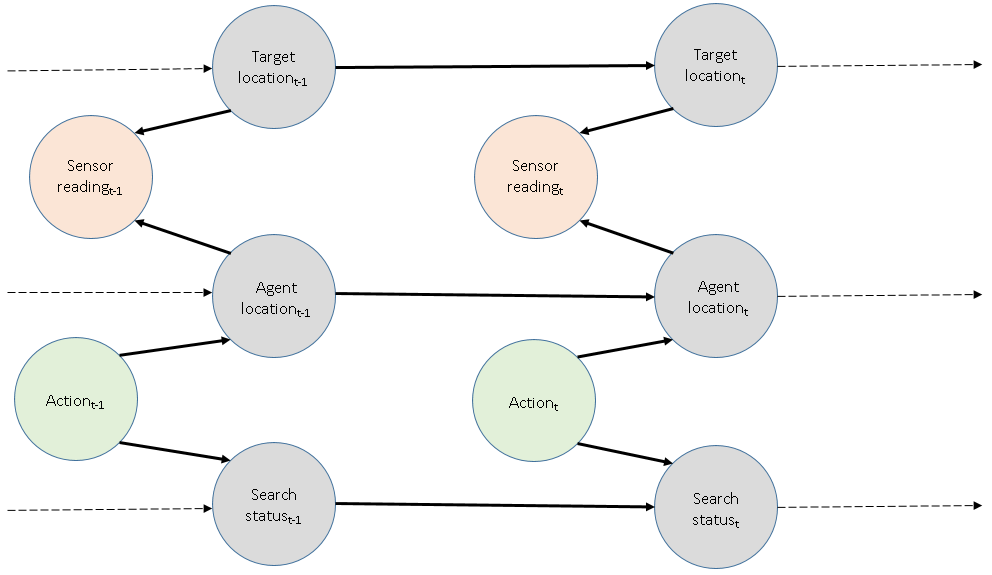
\includegraphics[width = 0.8\linewidth]{Chapters/MultiAgentTargetDetection/Figs/DBNWithMultipleHiddenState.PNG}
     \caption{First Version of the DBN representing the agent world model}
    \label{fig:FirstDBNUsed}
\end{figure}
A number of conditional probabilities are specified here in order to describe the factored joint distribution of the world model fully. The full tables are omitted as they are sparse. For brevity, we use the abbreviation Loc for Location.



\begin{figure}[H]
\scriptsize
\begin{equation}\label{eqn:EvidenceVarsProbs}
    %\centering
    p(SensorReading_t | AgentLoc_{t-1}, EvidenceLoc_{t-1})  = 
    \begin{cases}
    \alpha \quad \text{ if } SensorReading_t=1 \text{ and } EvidenceLoc_t \neq AgentLoc_t
    \\
    1-\beta \quad \text{ if } SensorReading_t=1 \text{ and } EvidenceLoc_t = AgentLoc_t
    \\
    \beta \quad \text{ if } SensorReading_t=0 \text{ and } EvidenceLoc_t \neq AgentLoc_t
    \\
    1-\alpha \quad \text{ if } SensorReading_t=0 \text{ and } EvidenceLoc_t \neq AgentLoc_t
    \end{cases}
    %
\end{equation}
\caption{Conditional Probability Distribution for the $Evidence$ Variable}
\end{figure}


\begin{figure}[H]
\scriptsize
\begin{equation}\label{eqn:TargetLocProbs}
    p(TargetLoc_{t} | TargetLoc_{t-1}) =
    \begin{cases}
    1 \quad \text{ if } TargetLoc_{t}=TargetLoc_{t-1}
    %agent returns correct target Loc.} 
    \\
    0 \quad \text { otherwise. }
    \end{cases}
\end{equation}
\caption{Conditional Probability Distribution for the $TargetLocation$ Variable}
\end{figure}





\begin{figure}[H]
\scriptsize
%\begin{equation}\label{eqn:SearchStatus}
    \begin{gather}\label{eqn:SearchStatus}
        p(SearchStatus_t | SearchStatus_{t-1}, Action_{t-1}) = \\
        \begin{cases}
        1 \quad \text{ if } SearchStatus_t = terminated\_x_i \text{ and } SearchStatus_{t-1} = terminated\_x_i 
        \\
        1 \quad \text{ if } Action_t = terminate\_x_i \text{ and } SearchStatus_{t-1}=ongoing \text{ and } SearchStatus_{t} = terminated\_x_i
        \\
        1 \quad \text{ if } Action_t = move\_x_i \text{ and } SearchStatus_{t-1}=ongoing \text{ and } SearchStatus_t=ongoing
        %agent returns correct target location.} 
        \\
        0 \quad \text { otherwise. }
        \end{cases}
    \end{gather}
%\end{equation}
\caption{Conditional Probability Distribution for the $SearchStatus$ Variable}
\end{figure}





\begin{figure}[H]
\scriptsize
    \begin{equation}\label{eqn:AgentLocation}
        p(AgentLoc_t | AgentLoc_{t-1}, Action_{t}) = 
        \begin{cases}
        1 \quad \text{ if } Action_t = move\_x_i \text{ and } AgentLoc_t = x_i
        \\
        1 \quad \text{ if } Action_t = terminate\_x_i \text{ and } AgentLoc_t = AgentLoc_{t-1}
        \\
        0 \quad \text{otherwise}
        \end{cases}
    \end{equation}
\caption{Conditional Probability Distribution for the $AgentLocation$ Variable}
\end{figure}


\normalsize
The semantics of the equations listed above is given here: 
\begin{enumerate}
    \item Equation \ref{eqn:EvidenceVarsProbs} uses two parameters, $\alpha$ and $\beta$, to represent the probability of making a false positive and false negative sensor reading, respectively. These are assumed to have been calculated by using pre-calibrated values of the sensor. This model is very flexible and does not stipulate any restrictions on the sensor other than that it must return a reading indicating that the target is present or not.
    \item  Equation \ref{eqn:TargetLocProbs} simply states that the location of the target does not change, even though it is hidden. It would be very easy to modify this to allow for moving target detection in the case of a non-static target.
    \item Equate \ref{eqn:SearchStatus} is also states a number of intuitive notions. The first line states that once the agent terminates the search, it remains over. The second line states that if the agent requests an ongoing search to terminate, then it does so deterministically. The third line states that if the agent chooses to move in an ongoing search, then the search remains ongoing.
    \item Equation \ref{eqn:AgentLocation} simply outlines that the agent moves to new locations deteministically. It also indicates that should the agent choose to terminate the search, then the environment enters a terminal state, indicating that the search is over.
\end{enumerate}


Note that despite the fact that some hidden state variables cannot be observed directly, it is still possible to infer their value exactly based on their starting state. For example, the position of the agent is a deterministic function of its actions and previous position. These variables could have been treated as variables that are internal to the agent rather than part of the hidden world state and many authors omit such variables for the sake of clarity.
\note{need to outline why I have included them - mainly because evidence probability depends on agent location as well as source location}


\subsubsection{Estimated State}
\workinprogress
Since the agent operates in a partially observable environment, the agent's internal state representation of the environment needs to take into account the fact that the current environment state is not certain. For this reason, a probability distribution over possible environment states is used by the agent to internally represent the environment state. The internal agent state is described mathematically by 
\[p(x_t | e_{1:t}, u_{1:t})\]
, which is the distribution of possible world states given all evidence and control actions up to the current time step, where $x_t$, $e_t$ and $u_t$ follow the conventions of being the hidden state variables, the evidence variables and the control action variables. The agent updates this state using the world model specified in the preceding chapter, using the filtering algorithm explained in section \ref{subsection:InferenceHMMDBN} of Chapter \ref{chapter:Background}. There are a couple of noteworthy points:
\begin{itemize}
    \item A distribution that has a single sharp peak would indicate that the agent believes that the target is at a specific location with high confidence. This is clearly preferred to a flat, uniform distribution representing uncertainty in relation to where the target might be.
    \item The only true source of uncertainty in the world state is introduced by the sensor. Therefore, analysis of this state representation in relation to the sensor model should provide insight into how the system performs.
\end{itemize}
In order to update the estimated state of the agent, the below equations are used, which are described in subsection \ref{subsection:InferenceHMMDBN}. For brevity $x_t$ denotes the hidden state variables, $e_t$ denotes the evidence variable and $u_t$ denotes the control action taken by the agent. The equations only describe the estimated state update for move actions, since if the agent terminates the search a terminal state is deterministically entered. The $SearchStatus$ variable is omitted from the equations since it only effects the equations if the $Action$ variable is to terminate the search.
\footnotesize
\begin{figure}[H]
\scriptsize
%\begin{equation}\label{eqn:SearchStatus}
    \begin{gather}\label{eqn:SearchStatus}
        p(AgentLoc_t = x, TargetLoc_t = y | e_{1:t}, u_{1:t}) = \\
        \begin{cases}
            \eta \alpha p(AgentLoc_{t-1} = x, TargetLoc_t = y | e_{1:t-1}, u_{1:t-1}) \text{ if $e_t$ is a positive reading and $AgentLoc_t \neq TargetLoc_t$} \\
            \eta \beta p(X_{t-1}=x_t | e_{1:t-1}, u_{1:t-1}) \text{ if $e_t$ is a negative reading and $Agent_loc_t$ = $TargetLoc_t$} \\
            \eta (1-\alpha) p(X_{t-1}=x_t | e_{1:t-1}, u_{1:t-1}) \text{ if $e_t$ is a negative reading and $Agent_loc_t \neq TargetLoc_t$} \\
            \eta (1-\beta) p(X_{t-1}=x_t | e_{1:t-1}, u_{1:t-1}) \text{ if $e_t$ is a positive reading and $Agent_loc_t$ = $TargetLoc_t$} \\
        \end{cases}
%\eta O_{t} T^{T} f_{1:t-1} 
    \end{gather}
\end{figure}
\normalsize


\subsection{Action Selection Strategies}\label{subsubsec:ActionSelection}
At each discrete time step the agent may either choose to terminate the search or move to a new location to take a measurement reading. The agent may choose which of these actions to perform based on its location, the search status and its internal representation of the environment, which are outlined in the preceding section. First we discuss how move actions are chosen, if the agent decides that the search should not be terminated at the current time step. We began by implementing some of the recommended basic search strategies outlined in the related works by \citeauthor{Chung2007ASearch} \cite{Chung2007ASearch} and \citeauthor{Waharte2010SupportingUAVs} \cite{Waharte2010SupportingUAVs}. These search methods are devised in order to optimize the agent's performance measure, which is set out in Section \ref{sssection:PerfMeas}. The results of applying these strategies are discussed in Section \ref{sec:SimulationResults}.\par 
%\note{In the following, might be good to mention the motivation in relation to the performance measure}
\textbf{Random Search}
This method serves as a baseline against which similar strategies can be compared. The agent simply chooses the next grid location to explore randomly from all possible grid locations. The expected number of moves needed to take a reading at all possible grid cells is given by the solution to the \textit{coupon collectors problem} \cite{Erdos1961OnTheory}, $nH_n$, where $H_n$ is the $n_{th}$ harmonic number and $n$ is the total number of grid cells, which gives a good idea of the expected amount of time that will be taken to conclude the search.

\textbf{$\epsilon$-Greedy Search}
A simple greedy search was implemented next, where the agent chooses to visit the grid cell with the highest estimated probability of containing the target in a localized region around the agent:
\footnotesize
\[
Action_t = \argmax_{NewLoc \in N(AgentLoc)}{p(TargetLoc = NewLoc, SearchStatus, AgentLocation| e_{1:t}, u_{1:t})}
\]
\normalsize
$N(AgentLoc)$ is a function that returns a neighborhood of locations around the agent's location and can be calibrated to trade off the cost of saccading between grid cells that may be far from each other against the cost of limiting the agents range to a narrow and possibly "cold" region.This method is designed bearing in mind that there may be motivation to explore some areas before others based on prior knowledge. 

%\textbf{$\epsilon$-greedy Search} Greedy search  simplest method to implement was an $\epsilon$-greedy action selection method, whereby the agent moves to the grid cell with the highest estimated probability in a pre-defined radius with probability 1-$\epsilon$ and a random grid cell in the pre-defined with probability $\epsilon$. This encourages the agent to exploit it's current know\par

\textbf{Saccadic Search}
This was proposed in \cite{Chung2007ASearch} and is a special case of $\epsilon$-greedy search. The idea is to mimic the behaviour of the human eye when looking at an image, whereby it "\textit{saccades}" from one salient feature to another. The consequence is that the most promising cells are explored at each time step, which means that the agent can be drawn to travel large distances in order to explore a peak in the spatial distribution given by the occupancy grid. Further details are given in \cite{Chung2007ASearch}.

\textbf{Sweep Search}
This strategy sweeps the region of interest systematically, aiming to take a reading at each grid cell an equal number of times while minimizing the total distance travelled. It then traverses this same path again in reverse order. This requires planning a trajectory in advance, which is often referred to in related literature as the \textit{complete coverage path}. Since the region to be swept is assumed to be a grid, where adjacent points are assumed to be equidistant, a number of heuristic solutions were available for use from Section \ref{sec:SceneSurveying}.\par

%\textbf{POMDP Based Search} 
%\note{Not sure if I should go into this at all. Work was done in understanding POMDPs and clearly the solution can be easily framed as a POMDP but my work stopped short in actually finding a solution to POMDP that works well}
%As outlined in 
%details. \par


\subsection{Search Termination}\label{subsubsec:SeachTerminationMethodology}

At each discrete timestep, the agent can either choose to move to a new grid location to record a sensor measurement or it can decide to terminate the search based on its estimated state of the environment. There is a trade-off in terminating the search early, which means that less time and resources are spent on continuing the search, versus the possibility of drawing misinformed conclusions from the search due to a lack of information. For example, if the agent receives a series of false positive readings at a given location, it could mistakenly choose to conclude that the target is present at a given location rather than sample further to gain confidence that it has correctly found the location of the target. Following this line of thinking, it is clear that a strategy needs to be devised to minimize the probability of drawing false conclusions, which is described in the performance measure set out in Section \ref{sssection:PerfMeas}.\par
\citeauthor{Pollock1971SearchInterfaces} outlines three commonly used criteria that can be used to make a decision whether to terminate the search or not: the \textit{Bayes Criterion}, which minimizes the expected cost per decision, the \textit{Minimax Criterion}, which chooses a decision which minimises the maximum expected cost and the \textit{Neyman-Pearson Criterion}, which uses a likelihood ratio test to determine the optimal decision to make \cite{Pollock1971SearchInterfaces}. These tests are proposed in the context of a target that is definitely present in the search region, but can be extended to incorporate the decision problem where the target may or may not be present. In addition, related work by \citeauthor{Chung2007ASearch} has addressed this problem using methods that use heuristics to make a decision whether to terminate the search or not \cite{Chung2007ASearch}. 

We ultimately choose to implement the Sequential Probability Ratio Test (SPRT), which is a hypothesis-testing framework developed by \citeauthor{Wald1950BayesProblems} to optimally deal with sequential decision problems, as opposed to traditional frameworks which assume that all the necessary data has been gathered prior to analysis \cite{Wald1950BayesProblems}. The background knowledge behind the SPRT can be found in Section \ref{subsec:SPRT}. An algorithm is also provided on how to perform this test in practice.
%The details of the proof of optimality of the SPRT is given in \cite{Wald1950BayesProblems} and we have outlined the details of how to perform hypothesis-testing using this framework in section <refer to the section>, along with the practical advantages and drawbacks of using it. 
We applied the SPRT algorithm to our problem to provide a search termination criteria using the following quantities: 
%In order to allow the agent to make a decision on whether to terminate the search or not, the following procedure was used: \note{Might be worthwhile simply outlining the algorithm}

\begin{gather}\label{eqn:SPRTQuantities}
H_0 : \text{The null hypothesis, the target is not present in the search region}\nonumber
\\ \nonumber
H_1 : \text{The alternative hypothesis, the target is present in the search region}\nonumber
\\ \nonumber
\alpha : \text{The maximum probability of making a type } \Romannum{1} \text{ error.} \nonumber
\\ \nonumber
\beta : \text{The maximum probability of making a type } \Romannum{2} \text{ error.}\nonumber
\\ \nonumber
\\ \nonumber
p_{0t} : \text{ The probability of observing the data $(e_1, ..., e_t)$ under the assumption of $H_0$} \nonumber
\\ \nonumber
p_{0t}=\sum_{loc=1}^{n} p(TargetLoc_t = loc, AgentLoc_t, SearchStatus_t| e_{1:t}, u_{1:t})\nonumber
\\ \nonumber
\\ \nonumber
p_{1t} : \text{ The likelihood of observing the data $(e_1, ..., e_t)$ under the assumption of $H_1$} \nonumber
\\ \nonumber
p_{1t}=p(TargetLoc_t = n+1, AgentLoc_t, SearchStatus_t | e_{1:t}, u_{1:t})\nonumber 
\end{gather}

$p_{0t}$ and $p_{1t}$ are calculated by using the evidence likelihood algorithm, which is described in detail in Section \ref{subsubsec:EvLikelihood}. The SPRT algorithm was then used at each timestep to decide whether to 
\begin{enumerate}
    \item Terminate the search accepting $H_0$, that the target is not present in the search region.
    \item Terminate the search accepting $H_1$, that the target is present in the search region. In this case, the target location with the highest estimated probability is returned as the target location.
    \item Continue the search, using the Action Selection Strategy described in Section \ref{subsubsec:ActionSelection}.
\end{enumerate}
In practice, we often took logarithmic transforms of the values used in the SPRT, to simplify some calculations and to be able to look at plots that are less heavily skewed and simpler to interpret.

\subsection{Analysis of Search Termination Criteria}
The two parameters, $\alpha$ and $\beta$ that the user needs to specify to perform the SPRT need to be chosen carefully and depend on the context of the search. As in the standard hypothesis testing context, it is important to consider the significance level and power of the test to ensure that they reflect the severity of drawing an incorrect conclusion \cite{IntroductionToMathematicalStatistics}. They can also help to perform analysis on how well the agent could perform, since setting a high threshold means that the agent may have to take a minimum number of samples at the correct target location in order to choose $H_0$ or $H_1$. \par

Figure \ref{fig:SPRTCutoffFunctionOfAlphaAndBeta} shows how A and B vary as functions of the parameters $\alpha$ and $\beta$ on a log scale
%\footnote{Tables of the values of A and B for varying for varying Type \Romannum{1} rates ($\alpha$) and Type \Romannum{2} ($\beta$) error rates may be referred to in Appendix \ref{chap:AppendixOne}.}. 
Tables of the values of A and B for varying for varying Type \Romannum{1} rates ($\alpha$) and Type \Romannum{2} ($\beta$) error rates may be referred to in Appendix \ref{chap:AppendixOne}.
If the log-likelihood ratio of the data lies in between the red and blue surfaces on the graph, another sample is taken. A projection of this plot is shown in Figure \ref{fig:VaryingSPRTParametersProjected1}:
\begin{enumerate}[label=(\alph*)]
    \item shows a plot of how varying the Type \Romannum{1} error rate $\alpha$ for a fixed Type \Romannum {2} error rate $\beta = 0.07$ affects the decision boundaries defined by A and B.
    \item shows a plot of how varying the Type \Romannum{2} error rate $\beta$ for a fixed Type \Romannum{1} error rate $\alpha = 0.1$ affects the decision boundaries defined by A and B.
\end{enumerate}

Figures \ref{fig:SPRTCutoffFunctionOfAlphaAndBeta} and \ref{fig:VaryingSPRTParametersProjected1} reflect the intuition behind the decision boundaries. The lower the probability of making either a Type \Romannum{1} or Type \Romannum{2} error, the further apart the decision boundary becomes, meaning the likelihood ratio must be very far apart from 1, which appears as 0 on the log scale. A likelihood ratio of 1 indicates maximum uncertainty. It is also possible to see that the surfaces meet when $\alpha=0.5$, $\beta=0.5$, which reflects the fact that immediately terminating the search will give a 0.5 probability of returning a false positive or false negative. \par

\note{Might be better off editing these images with explicit labels showing regions in which H0 and H1 will be accepted.}
Figure \ref{fig:VaryingSPRTParametersProjected2} shows the regions in which the SPRT will elect to take another sample (the green shaded region), to accept $H_0$, the upper red shaded region, and to accept $H_1$, the lower red shaded region. The blue line shows the log-likelihood ratio of $\frac{(e_{1:t} | H_0)}{p(e_{1:t} | H_1)}$ as a function of the agent belief that the target is present in the search region. 
\note{This is not really clear, should exaggerate this more}
Note that since the values of $\alpha$ and $\beta$ are significantly smaller in Figure \ref{fig:VaryingSPRTParametersProjected2} (b) than in Figure \ref{fig:VaryingSPRTParametersProjected2} (a), the acceptance region for $H_0$ and $H_1$ are significantly smaller in (b) than in (a).

\par
%varying the type \Romannum{1} error rate for a fixed type \Romannum{2} error rate affects the upper and lower threshold for cutting off the search. Figure \ref{fig:SPRTVaryingT2} shows how the varying the type \Romannum{2} error rate for a fixed type \Romannum{1} error rate affects the upper and lower threshold for cutting off the search. Note that as the varying error rate increases on the x-axis, the decision boundaries come closer together, reflecting the intuition that we are more willing to accept a mistaken conclusion.
%\begin{figure}
%    \centering
%    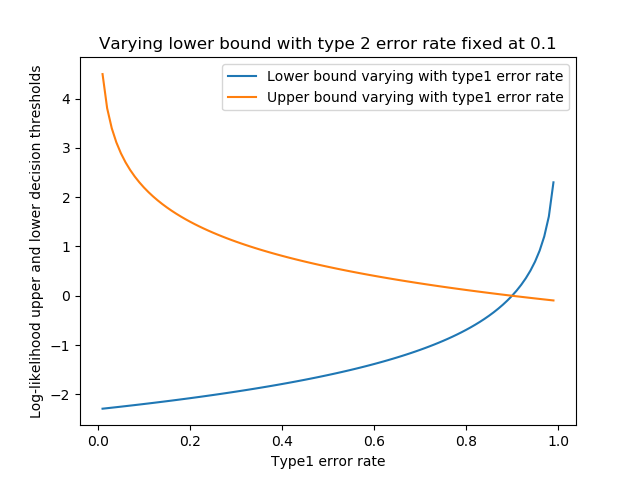
\includegraphics[width = 0.75\linewidth]{Chapters/MultiAgentTargetDetection/Figs/SearchTermination/SPRTDecisionThresholdVaryingT1ErrorRate.png}
%    \caption{The Log-likelihood upper and lower threshold for a varying type \Romannum{1} error rate and fixed type \Romannum{2} error rate.}
%    \label{fig:SPRTVaryingT1}
%\end{figure}

%\begin{figure}
%    \centering
%    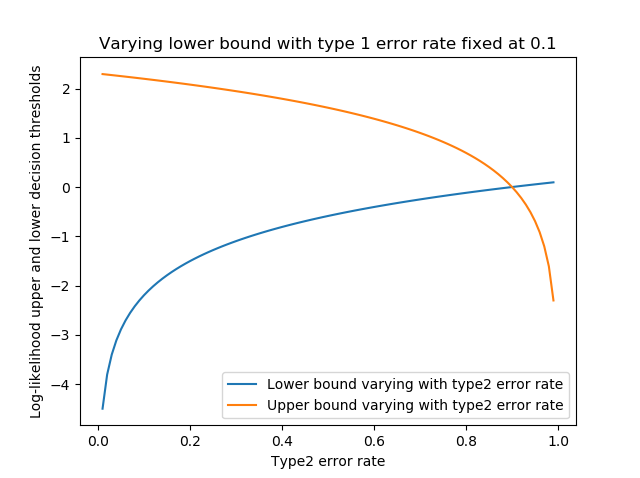
\includegraphics[width = 0.75\linewidth]{Chapters/MultiAgentTargetDetection/Figs/SearchTermination/SPRTDecisionThresholdVaryingT2ErrorRate.png}
%    \caption{The Log-likelihood upper and lower threshold for a varying type \Romannum{2} error rate and fixed type \Romannum{1} error rate.}
%    \label{fig:SPRTVaryingT2}
%\end{figure}

%Show how A and B vary for a fixed T1 or T2 error rate.
\begin{figure}[H]
    \centering
    \subfloat[Varying T\Romannum{1} error rate for a fixed T\Romannum{2} error rate]{{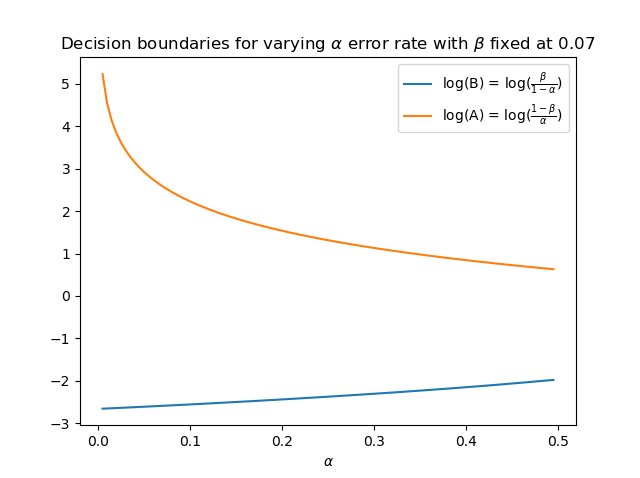
\includegraphics[width=11cm]{Chapters/MultiAgentTargetDetection/Figs/SearchTermination/AAndBVaryingWithAlpha.png} }}%
    \qquad
    \subfloat[Varying T\Romannum{2} error rate and fixed T\Romannum{1} error rate]{{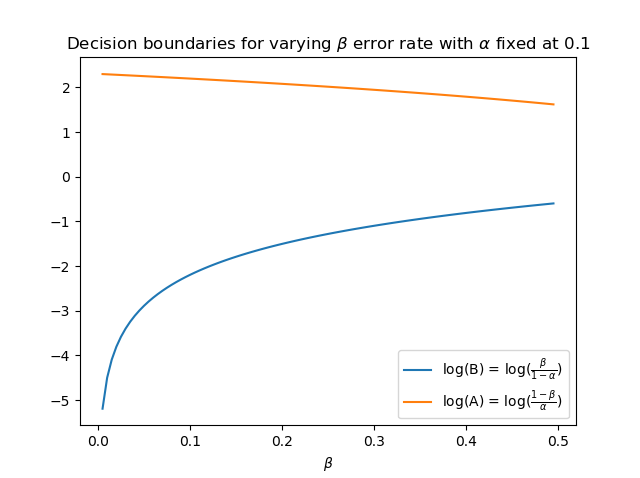
\includegraphics[width=11cm]{Chapters/MultiAgentTargetDetection/Figs/SearchTermination/AAndBVaryingWithBeta.png} }}%
    \caption{Upper and lower values of A and B for varying error rates. Values are shown on a log scale}%
    \label{fig:VaryingSPRTParametersProjected1}%
\end{figure}


%3-Dimensional plot to show how A and B vary with alpha and beta
\begin{figure}[h]
    \centering
    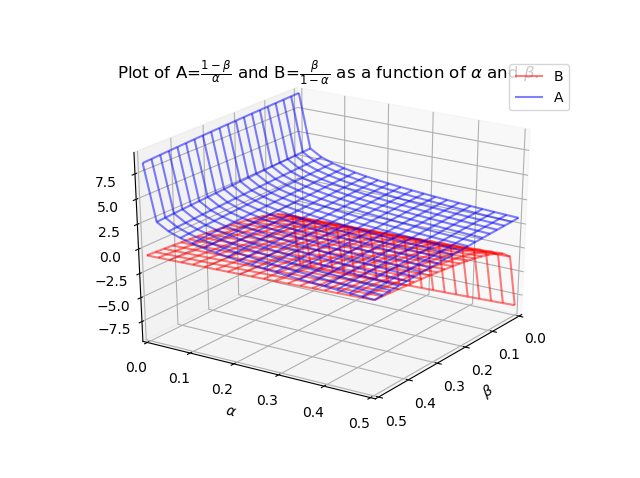
\includegraphics[width = 0.78\linewidth]{Chapters/MultiAgentTargetDetection/Figs/SearchTermination/AandBAsFunctionOfAlphaAndBetaLogTransform.png}
    \caption{The upper and lower SPRT bounds for acceptance and rejection of $H_0$, as functions of the significance and power of the test. Values are shown on a log scale.}
    \label{fig:SPRTCutoffFunctionOfAlphaAndBeta}
\end{figure}


%\begin{figure}
%    \centering
%    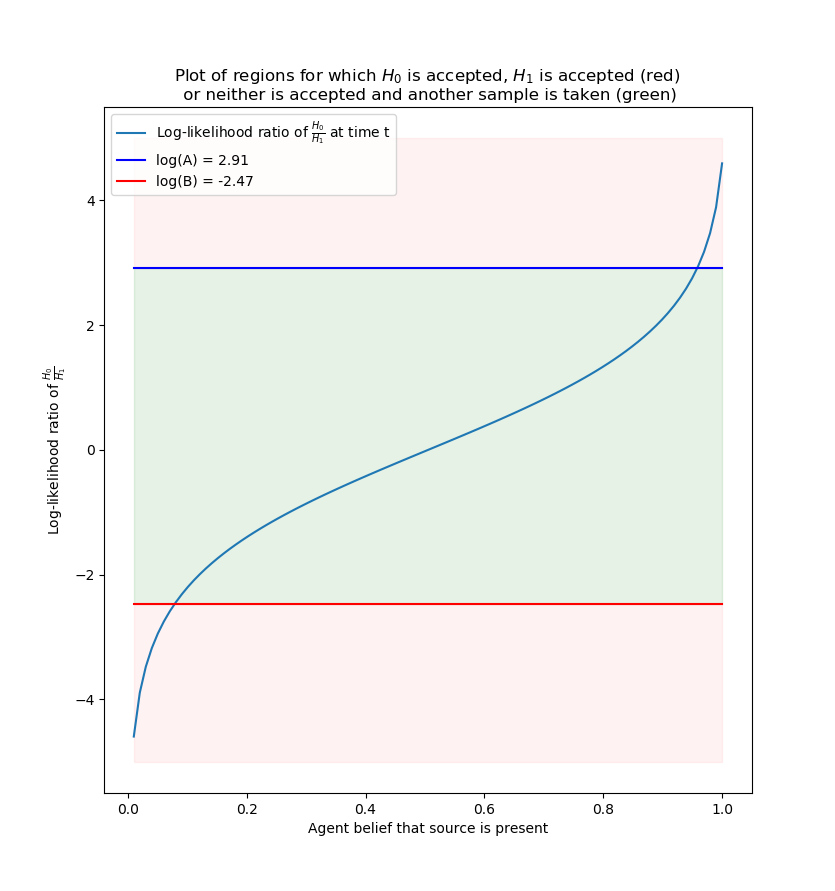
\includegraphics[width = 0.75\linewidth]{Chapters/MultiAgentTargetDetection/Figs/SearchTermination/CutoffRegions.png}
%    \caption{The cut-off regions of the SPRT for $\alpha=0.05$, $\beta=0.08$ as a function of agent belief in whether target is present or not. Values are shown on a log scale.}
%    \label{fig:SPRTLogLikelihoodRatio}
%\end{figure}

%showing how A and B create upper and lower limits for terminating the search
\begin{figure}[H]%
    \centering
    \subfloat[SPRT cut-off regions for $\alpha=0.05$, $\beta=0.08$]{{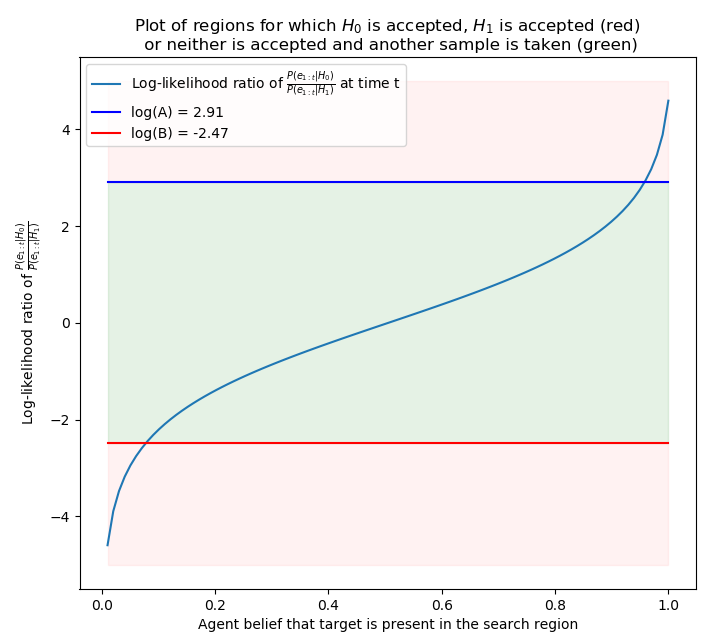
\includegraphics[width=11.5cm]{Chapters/MultiAgentTargetDetection/Figs/SearchTermination/CutoffRegionsAlphaPointZeroFiveBetaPointZeroEight.png} }}%
    \caption{} \label{fig:SPRTProjected1}
    %\qquad
\end{figure}
\begin{figure}[H]\ContinuedFloat
    \centering
    \subfloat[SPRT cut-off regions for $\alpha=0.01$, $\beta=0.02$ \label{fig:SPRTProjected2}]{{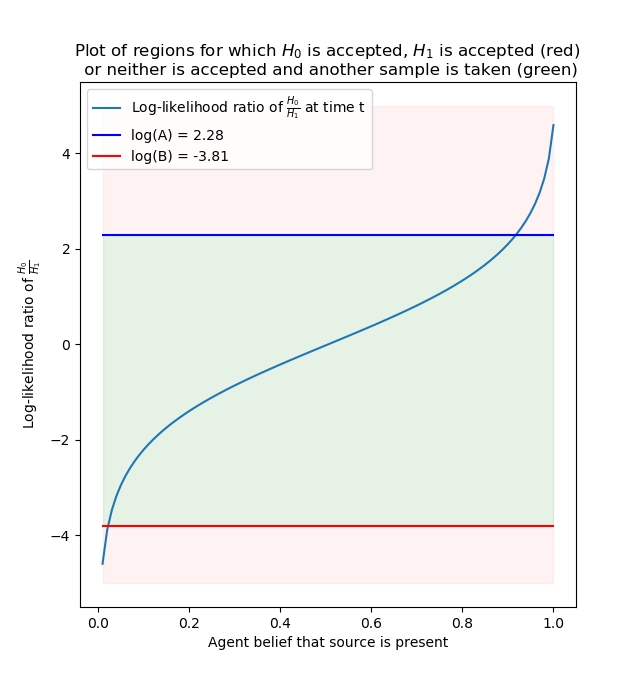
\includegraphics[width=11.5cm]{Chapters/MultiAgentTargetDetection/Figs/SearchTermination/CutoffRegionsAlphaPointOneBetaPointZeroTwo.png} }}%
    \caption{The cut-off regions of the SPRT for (a) $\alpha=0.05$, $\beta=0.08$ and (b) $\alpha=0.01$, $\beta=0.02$ as a function of agent belief in whether target is present or not. Values are shown on a log scale.}%
    \label{fig:VaryingSPRTParametersProjected2}%
\end{figure}



\note{maybe move tables to appendix}














\subsection{Agent Function Architecture}\label{subsec:AgentFNArch}
\note{This section shows how the agent function is implemented. Diagram shows how DerivedOccupancyGridAgent actually operates.}
Putting together the components outlined so far in this chapter, we end up with an agent function that is shown in Figure \ref{fig:BasicAgentArchitecture}. 

\note{Fix this figure}
\begin{figure}
    \centering
    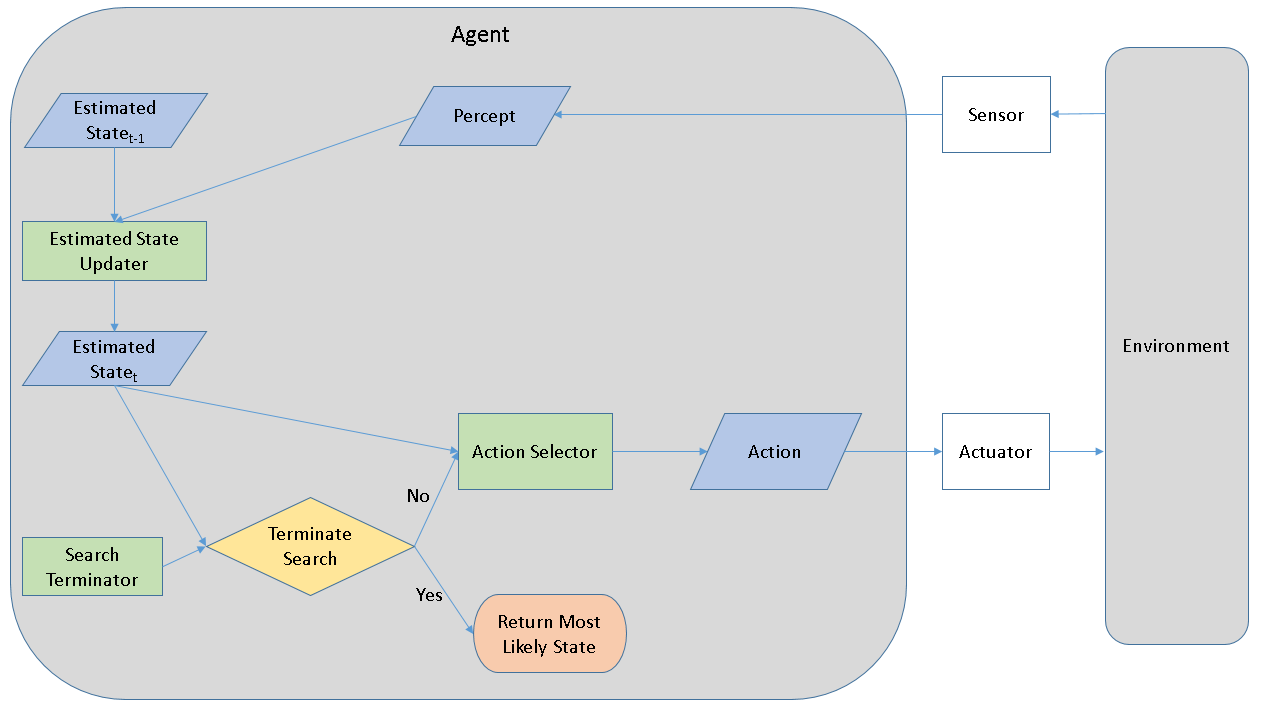
\includegraphics[width = 0.75\linewidth]{Chapters/MultiAgentTargetDetection/Figs/AgentFnArchitecture/BasicAgentFunctionNoCommunication.PNG}
    \caption{The structure of the agent function.}
    \label{fig:BasicAgentArchitecture}
\end{figure}


The diagram outlines how the agent interacts with its environment and abstracts away technical details such as the search status. This is a concrete version of the model-based reflex agent outlined in \cite[P~.51]{AIAMA}. The estimated state update rules are applied as outlined in the previous sections in this chapter. Algorithm \ref{alg:SingleTargetLocalisation} shows the algorithm which describes the agent function.
\note{might be able to bulk this up a bit, come back to it}



\begin{algorithm}{}
\caption{Single Target Localisation Algorithm}
\label{alg:SingleTargetLocalisation}

\begin{algorithmic}[1]
\renewcommand{\algorithmicrequire}{\textbf{Input:}}
\renewcommand{\algorithmicensure}{\textbf{Output:}}
%Input
\REQUIRE $ \newline initial\_estimated\_state = P(x_{0} | e_{0}, u_0), \quad \text{ The initial distribution of the estimated state}
\newline select\_action, \quad \text{Returns an action given an estimated state}
\newline estimated\_state\_updater, \quad \text{Returns the updated estimated state given the current} \newline \text{ estimated state, a percept and an action}
\newline SPRT, \quad \text{An object calibrated with a specified Type \Romannum{1}, Type \Romannum{2} error which has a method to implement} \newline \text{ the SPRT and an attribute which returns the result of the application of the SPRT.}
$
%Output
\ENSURE  $\newline \text{The grid cell containing the source, } x_i \text{ for } i \in \{1, ..., N\}, \text{ or } x_{N+1} \text{, indicating} \newline \text{ the source is not present}$

\hfill\pagebreak

\STATE $estimated\_state$ $\leftarrow$ $initial\_estimated\_state$
\WHILE{not $SPRT.should\_terminate\_search(estimated\_state)$}
\STATE $action \leftarrow select\_action(estimated\_state)$
\STATE $perform\_action(action)$
\STATE $percept \leftarrow get\_percept()$
\STATE $estimated\_state \leftarrow estimated\_state\_updater(estimated\_state, percept, action)$
\ENDWHILE
\RETURN $\argmax_{x_i}{p(x_i | e_{1:t}, u_{1:t}) = \argmax estimated\_state}$
\end{algorithmic} 
\end{algorithm}

\subsection{Extensions to the Basic Agent}
The agent design outlined in the preceding sections of this chapter addresses the problem outlined in Section \ref{subsec:ProbDescription},  following the assumptions outlined in Section \ref{subsec:initalAssumptions}. As mentioned in Section \ref{subsec:initalAssumptions}, some of these assumptions are not realistic, which we address in this section. \par

\subsubsection{Localising Multiple Targets}
The first assumption that we address is that there are either zero or one targets to be localised. In many applications, this is a very unrealistic assumption. For example, the ROCSAFE project (outlined in section \ref{sec:ROCSAFEBG}), which motivates this work, aims to apply object detection algorithms to aerial images in order to avoid the need to send a crime scene investigator into a hazardous scenario in order to verify the presence of a potential source of evidence.\note{check the above sentence is consistent with the Background} An assumption that is much more valid is that there are a maximum of $k$ unknown sources present in the search region, which addresses the general case for the ROCSAFE \note{should ROCSAFE be in italics?} project.\par

\note{May need to go into more detail here since people without a background in probability might not understand implications of high-dimensional joint distribution}
The main issue that arises when including \textit{multiple} targets in the hidden state, $X_t$, is that there is an exponential increase the dimensionality of the hidden state for each new target added. This means that maintaining an estimate of the state quickly becomes infeasible, since the run time of the forward algorithm detailed in section \ref{subsubsec:filteringDBN} is dependent on the square of the size of the joint distribution of the hidden state variables, $X_t$ and the memory requirements for maintaining the estimated state also depend on the dimensionality of the joint distribution of the hidden state. See section \ref{subsubsec:filteringDBN} for details of the filtering algorithm.


Section <reference lit review> of the literature review outlines a number of techniques that have been applied by other researchers in this domain in order to deal with the case of multiple targets. \note{maybe should leave all of this to lit. review and just outline what I did.} Related work \cite{Waharte2009CoordinatedUAVs} proposed to use an approach commonly used with occupancy grids, which is that every grid cell may or may not contain a target, independent of all other grid cells. This technique is often referred to as \textit{mapping} when the location of the agent is known. This is generally described in \cite[P.~284]{Thrun:2005:ProbabilisticRobotics}. Rather than maintain a multinomial distribution for $TargetLocation_{t-1}$, as was the case in the work outlined in this chapter, we create a new binary random variable representing a target being present or not in each grid cell, denote $m_i$ for $i \in {1,...,N}$. We denote m as the joint distribution of these random variables. 

A suitable DBN for this approach is shown in figure <>. This


In the case, estimating the joint distribution is not hard, since This results in a greatly simplified state estimate update equation, where the probability of the target being located in a grid cell does not change unless the observation was made in that grid cell. The major drawback of this approach is that there is no clear way to apply the SPRT, hence there is no clear way to decide when to terminate the search. 


stems from the fact that this assumption induces a simple dependence relation between grid cells, for which the update rule \ref{eqn:SearchStatus} can 


The first method, which is very commonly taken when using an approach that uses occupancy grids \cite{Elfes1989UsingNavigation}, is to assume that grid cells are indeped


\section{Simulation Results}

%\note{from c\&B analysis of sequential decision making}
%\note{Consider the following setting, where a single stationary tar-get is possibly located in a10×10 search region that is depicted in Fig. 5. The initial aggregate beliefB(0) is distributed among theC= 100 cells,  where  the  height  of  the  bars  in  each  cell represents the individual cell belief values, i.e., the probabilityp0cthat the target is present in a given cell, i.e.,c in {1,...,C} . SupposeB(0) = 0.75 ,  which  corresponds  to  an  initial  likeli-hood of 75\% that the target is truly present inA at the beginning of the search process. We examine the evolution of the search decision employing the different search strategies that are presented in the previous section. The search problem parameters that are used for the simulation studies, which are presented in this section, are tabu-lated in Table I. Simulations were allowed to run to completion (i.e., a decision was made), and statistics were calculated over N= 10 000 simulation replications. The values for the detec-tion errors, i.e.,alpha and beta , were chosen to reflect a representative sensor, such as a visual camera that provides aerial imagery in an outdoor and cluttered environment, which could be further calibrated empirically, e.g., by the sensor’s receiver operating characteristic (ROC) curve. Fig.  6  illustrates  the  evolution  of  the  belief  map  as  a search  agent  that  employs  the  myopic  search  strategy  thatmoves through the search region for the given search problem parameters. The searcher attempts to inspect or “clear” cells with the highest cell belief values, which, for the example bimodal belief distribution, requires visiting one peak followed by explo-ration of the other. Note that false-positive and false-negative detections  occur  throughout  the  search  process,  although  the searcher eventually arrives at the true location of the target and correctly terminates the search}


%note{From C\&B Analysis of sequential decision-making using prob. search. Consider a bounded discretized search areaA , which is de-fined byC disjoint cells. This discrete representation can charac-terize numerous environment types of diverse spatial scale, such as open areas that are relevant to maritime search operations, cluttered regions, such as obstacle-filled arenas, or structured environments, such as rooms and hallways in a building. Other factors, which include the geometry and extent of the searcher’s sensor footprint, and the size of the sought object, or other op-erational considerations (e.g., existing coordinates or reference systems) can also govern the specific cellular decomposition of the search area}

%\note{More general sensor models that account for additional spatial and/or temporal dependences be-cause  of  clutter  (indoor)  or  terrain  and  atmosphere  (outdoor) can  be  constructed  (e.g.,$\alpha$ s(k),kand $\beta$ s(k),k )  but  is  deferred for future study}


%note{In other words, the greater hindrance to deciding that a target is present in the search cell is the false-positive detection probabil-ity, since false alarms tend to prevent the searcher from “trust-ing” its positive observation. In contrast, if the missed detection probability is high, then the searcher cannot declare the search cell empty of the target with high confidence without expending multiple observations in the c}


The results presented in this section were generated by running Monte Carlo simulations of the search procedure, since finding a closed-form solution to the mean \textbf{T}ime \textbf{T}o \textbf{D}ecision (TTD) is not readily available in the general case \cite{Chung2012AnalysisStrategies}. We simulated the grid, the agents and the targets in order to evaluate the performance of the system.
%and to analyse how modifying search parameters affects the outcome.
We present statistics related to the Monte Carlo simulations, which reveal how modifying parameters of the search procedure affect the outcome. For each set of parameters in tables \ref{table:VaryingPriorDistribution}, \ref{table:VaryingInitialBelief}, \ref{table:MiscalibratedSensor}, \ref{table:MultipleTargetEGSweep}, \ref{table:MultipleTargetSaccadicRandom} and \ref{table:VaryingNumberOfAgents} we ran 5000 simulations, which finish when the agent (or agents) terminates the search. The parameters that we vary in the simulations are: 
\begin{enumerate}
    \item The prior belief distribution of each agent.
    \item The initial cumulative belief that the target is present in the region.
    \item The sensor model false positive rate and false negative rate.
    \item The number of targets present in the region.
    \item The number of agents participating in the search.
\end{enumerate}
The results of the simulations show how varying these parameters and suggest how to set them to achieve a desired result. We focus on the most commonly reported metrics in the literature, which are related to the distribution of time to decision \cite{Chung2012AnalysisStrategies}, \cite{Waharte2010ProbabilisticUAVs}, \cite{Waharte2010SupportingUAVs}, \cite{Lau2007OptimalEnvironments}. We also report on the rate at which incorrect target locations are returned and the rate at which the agents incorrectly conclude that the target is not present. 

\par For each of the simulations, we arbitrarily chose to use the SPRT cutoff criteria with the upper Type \Romannum{1} error probability set to 0.1 and the upper Type \Romannum{2} error probability set to 0.15. In practice, this meant the agent would terminate the search if its cumulative belief that the target was present exceeded 0.895 or subceeded 0.143. We generated simulated sensor readings using arbitrarily chosen values of the false positive rate = 0.2 and a false negative rate = 0.15. For each simulation run, we generated random starting locations for the agents and targets in a uniformly spaced 10 $\times$ 10 grid. Unless specified otherwise, we use the following default parameters: sensor model false negative rate = 0.15, sensor model false positive rate = 0.2, initial belief distribution = uniform, initial cumulative belief target is present = 0.5, number of targets present = 1, number of active agents = 1, the $\epsilon$-greedy search has $\epsilon$=0.2 and a neighborhood radius of 4. Histograms showing the results of running the simulation with varying parameters are shown in Appendix \ref{chap:AppendixTwo}.

\subsection{Simulation Results Using a Single Agent}\label{subsec:SingleAgentSingleSourceResults}
\subsubsection{Varying the initial distribution of the agent belief}\label{subsubsec:VaryingPrior}

%\begin{landscape}
%\centering
%\vspace*{\fill}
\begin{table}[h!]
    \centering
    \begin{tabular}{| >{\centering} m{18mm} | >{\centering}m{22mm} | >{\centering}m{22mm} | >{\centering}m{22mm} | >{\centering}m{20mm} | m{20mm} <{\centering}|}
    \hline
       Strategy & Initial Belief Distribution & Mean TTD & Sample SD[TTD] & False Negative Rate & Proportion Incorrectly Localised \\
        \hline
        $\epsilon$-Greedy & Uniform & 112.93 & 62.38 & 0.152 & 0.040 \\
        $\epsilon$-Greedy & Gaussian & 21.68 & 20.44 & 0.0296 & 0.0118 \\
        \hline
        Sweep & Uniform & 601.57 & 183.45& 0.1254 & 0.0454 \\
        Sweep & Gaussian & 464.48 & 185.54 & 0.0832 & 0.0294 \\
        \hline
        Saccadic & Uniform & 98.83 & 56.13 & 0.1588 & 0.037 \\
        Saccadic & Gaussian & 14.558 & 18.75 & 0.0338 & 0.0114 \\
        \hline
        Random & Uniform & 629.55 & 282.95 & 0.1368 & 0.0336 \\
        Random & Gaussian & 501.83 & 268.45 & 0.0792 & 0.0308 \\
        \hline
    \end{tabular}
    \caption{Results of running the target localisation simulation with a Uniform initial belief distribution and Gaussian initial belief distribution for each implemented search strategy.}
    \label{table:VaryingPriorDistribution}
\end{table}
    
Table \ref{table:VaryingPriorDistribution} displays the results of running a simulation with a single agent and a single target while varying the initial belief distribution that the target is present in the search region. 
%The following parameters are fixed: Simulated Sensor False Negative Rate = 0.15, Simulated Sensor False Positive Rate = 0.2, Sensor model False Negative Rate = 0.15, Sensor Model False Positive Rate = 0.2, Initial belief that target is present in region = 0.5, SPRT Type \Romannum{1} error rate = 0.1, SPRT Type \Romannum{2} error rate = 0.15.
%\begin{itemize}
%    \item Simulated Sensor False Negative Rate = 0.15
%    \item Simulated Sensor False Positive Rate = 0.2
%    \item Sensor model False Negative Rate = 0.15
%    \item Sensor Model False Positive Rate = 0.2
%    \item Initial belief that target is present in region = 0.5
%    \item SPRT T\Romannum{1} error rate = 0.1, SPRT T\Romannum{2} error rate = 0.15.
%\end{itemize}
\begin{figure}
\centering
    \subfloat[Uniform initial belief distribution]{{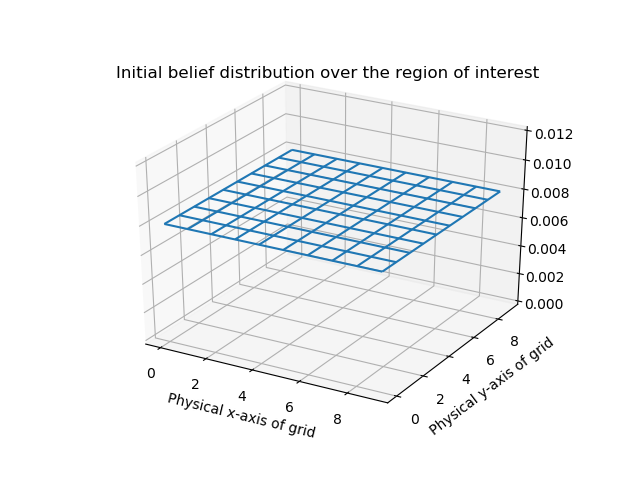
\includegraphics[width=6cm]{Chapters/MultiAgentTargetDetection/Figs/Results/Prior/Uniform/UniformInitialDistribution.png} }}%
    \qquad
    \subfloat[Gaussian initial belief distribution]{{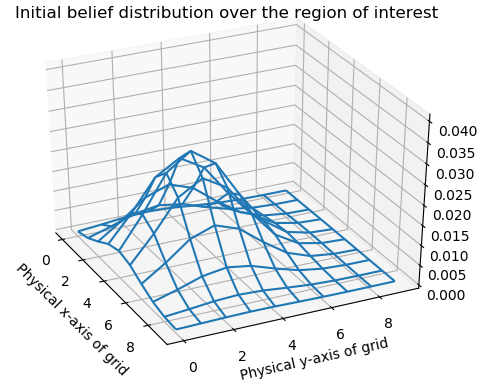
\includegraphics[width=6cm]{Chapters/MultiAgentTargetDetection/Figs/Results/Prior/Gaussian/GaussianInitialDistribution.png} }}%
    \caption{Initial belief distributions}%
    \label{fig:initialBeliefDistribution}%
\end{figure}
For each search strategy, we ran the simulation with both a Uniform and Gaussian initial belief distribution. The Gaussian mean coincided with the target location and the covariance matrix was $\begin{pmatrix} 3 & 0\\ 0 & 3\end{pmatrix}$, which is visualised in Figure \ref{fig:initialBeliefDistribution}. This represents a correct suspicion about the location of the target, which is the case in many scenarios where some prior information may suggest clues to the target location. As expected, for all of the search strategies the expected time until a decision reduces dramatically when using the Gaussian prior relative to the Uniform prior. 
%In the case of the two non-adaptive search methods (random and sweep), the effect is lessened as the search process is not influenced by new observations. 
Since the shape of the Gaussian distribution is aligned more closely to the true distribution that the Uniform distribution, it takes fewer samples to reach a sufficiently peaked distribution to reach the acceptance region for the SPRT. 
%This is visible by examining the evolution of the cumulative agent belief that the target is present in the region, shown in figures x and y.

\par It can also be seen that the false negative rate (the rate at which the agent incorrectly concludes that the target is not present in the region) drops in the case of the Gaussian prior relative to the uniform prior. This is also a result of using a prior distribution that matches the shape of the true distribution, since it requires a significant number of false positive/negative samples to modify the distribution enough to reach a negative conclusion.

%This is due to the unbiased sampling method of the non-adaptive strategies, which 

%but is higher for the non-adaptive search strategies since they are unbiased while sampling grid locations.
   

%    \hline
%    \multicolumn{2}{c}{Initial Discretised Gaussian Distribution of Belief Over Grid Cells (random mean, covariance matrix = [[], []]}\\
%    \hline

%\textbf{Gaussian Initial Belief Distribution (Mean coinciding with true target location)}
%\begin{table}[h!]
%    \centering
%    \begin{tabular}{| >{\centering} m{18mm} | >{\centering}m{20mm} | >{\centering}m{18mm} | >{\centering}m{20mm} | >{\centering}m{20mm} | m{20mm} <{\centering}|}
%    \hline
%       Strategy & Initial Belief Distribution & E[Time To Decision] & SD[Time To Decision] & False Negative Rate & Proportion Incorrect Localised \\
%        \hline
%        $\epsilon$ -Greedy & Gaussian & 21.68 & 20.44 & 0.0296 & 0.0118 \\
%        Sweep & Gaussian & 464.48 & 185.54 & 0.0832 & 0.0294 \\
%        Saccadic & Gaussian & 14.558 & 18.75 & 0.0338 & 0.0114 \\
%        Random & Gaussian & 501.83 & 268.45 & 0.0792 & 0.0308 \\
%    \hline
%    \end{tabular}

%  \caption{Results of running the target localisation simulation with a  uniform initial belief distribution and Gaussian initial belief distribution. p(T \Romannum{1}) = The probability of making a type \Romannum{1} error using the SPRT, p(T \Romannum{2}) = The probability of making a type \Romannum{1} error using the SPRT, Sim. FPR = The simulated false positive rate of the sensor, Sim. FNR = The simulated false negative rate of the sensor, E[TTD] = The expected amount of timesteps until a decision is made, Prec. = precision, Rec. = Recall. }\label{table:PriorGaussian}
%\end{table}





%\begin{landscape}

%\end{landscape}



































\break

\subsubsection{Varying the cumulative initial belief that the target is present in the search region}\label{subsubsec:VaryingPrior}
This experiment explored the consequences of varying the initial cumulative probability that the source is present. The cumulative probability of target presence reflects knowledge of likely the target presence is, prior to any evidence being gathered. We chose the parameters to reflect the cases where the search team do not believe it is unlikely that the target is present (0.25), it is equally likely that it is present as not present (0.5) and that it is likely that the target is present (0.75).

\begin{table}[H]
    \centering
    \begin{tabular}{| >{\centering} m{18mm} | >{\centering}m{24mm} | >{\centering}m{18mm} | >{\centering}m{20mm} | >{\centering}m{20mm} | m{20mm} <{\centering}|}
    \hline
       Strategy & Initial Belief Target Present & Mean TTD & Sample SD[TTD] & False Negative Rate & Proportion Incorrectly Localised \\
        \hline
        $\epsilon$-Greedy & 0.25 & 87.6214 & 30.9801 & 0.487 & 0.009 \\
        $\epsilon$-Greedy & 0.5 & 112.93 & 62.38 & 0.152 & 0.040 \\
        $\epsilon$-Greedy & 0.75  & 114.9276 & 81.9386 & 0.0396 & 0.1346 \\
         \hline
        Sweep & 0.25 & 520.4050 & 212.5122 & 0.4292 & 0.0118 \\
        Sweep & 0.5 & 601.57 & 183.45& 0.1254 & 0.0454 \\
        Sweep & 0.75 & 485.3650 & 242.1377 & 0.0326 & 0.1586 \\
        \hline
        Saccadic & 0.25 & 75.8320 & 29.8345 & 0.5054 & 0.0064 \\
        Saccadic & 0.5 & 98.83 & 56.13 & 0.1588 & 0.037 \\
        Saccadic & 0.75 & 100.1332 & 74.3883 & 0.0392 & 0.1418 \\
        \hline
        Random & 0.25 & 539.3802 & 267.6280 & 0.4284 & 0.0074 \\
        Random & 0.5 & 629.55 & 282.95 & 0.137 & 0.0336 \\
        Random & 0.75 & 538.0904 & 325.6283 & 0.035 & 0.1538 \\

    \hline
    \end{tabular}

  \caption{Results of running the target localisation simulation with a varying cumulative initial belief that the target is present in the search region.}\label{table:VaryingInitialBelief}
\end{table}

\begin{figure}[H]
\centering
    \subfloat[Belief for sweep search prematurely drops below the lower SPRT threshold with initial cumulative belief 0.25.]{{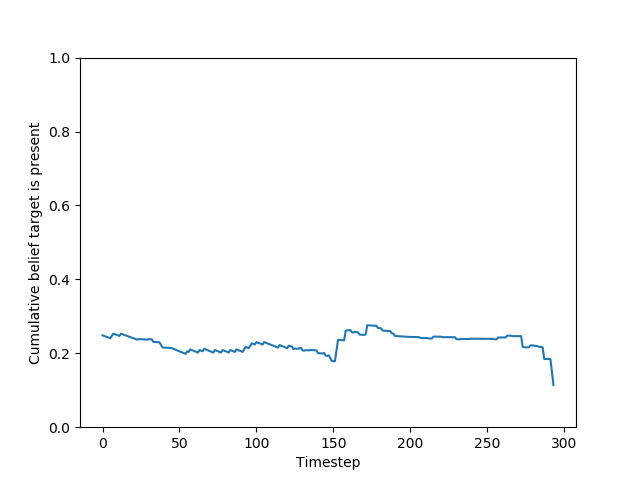
\includegraphics[width=7.4cm]{Chapters/MultiAgentTargetDetection/Figs/Results/BeliefEvolution/Sweep25InitialBelief/BeliefEvolution1.png} }}%
    \subfloat[Belief for sweep search does not prematurely drop below the lower SPRT threshold with initial cumulative belief 0.75.]{{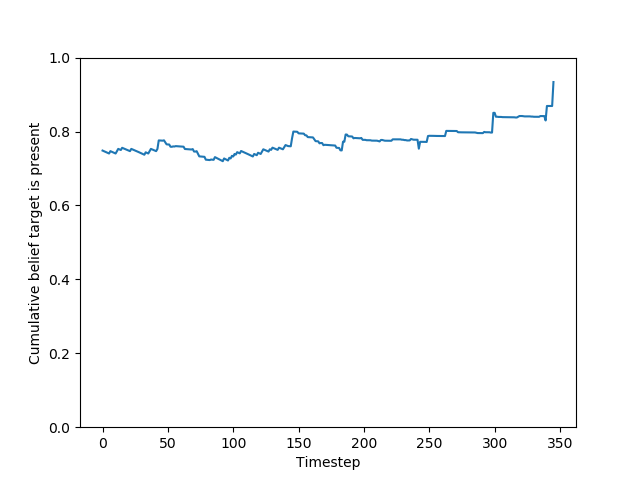
\includegraphics[width=7.4cm]{Chapters/MultiAgentTargetDetection/Figs/Results/BeliefEvolution/Sweep25InitialBelief/BeliefEvolution4.png} }}%
    \caption{Sample runs showing the effect of varying the agent's initial cumulative belief that the target is present}%
    \label{fig:initialCumulativeBelief}%
\end{figure}

Table \ref{table:VaryingInitialBelief} displays the results of running a simulation with a single agent and a single target while varying the agent's cumulative initial belief that the target is present in the search region. We discuss the results in relation to the adaptive and non-adaptive search methods:
\begin{enumerate}
    \item The results show that for the non-adaptive Sweep and Random search strategies, the mean TTD decreases when the initial belief that the target is present is set to both 0.25 and 0.75. In the case of the initial 0.25 belief value, the lower bound on the number of necessary observations before a conclusion can be drawn is found to be 62 consecutive negative observations at distinct locations. This would cause the SPRT to determine the target is not present. It is not likely for this to happen for the given parameters, since the sensor will generate false positive at a rate of 0.2, but there are much more likely scenarios that occur which cause the search to terminate early, for example observing 88 negative observations and 16 positive observations.
    %or 1 positive observation and 71 negative observations at distinct locations to pass the threshold(in the absence of any positive observations). Since there are 100 possible starting locations for the source, this is a likely scenario and
    \par The search terminates prematurely in a high proportion of cases, before a significant number of positive observations are observed to move the cumulative belief that the target is present away from the lower decision boundary. This can be observed in Figure \ref{fig:initialCumulativeBelief}, where on the left hand side there are not a sufficient number of positive observations to stop the search from terminating early. In the case of the 0.75 initial belief value, fewer positive observations are required to reach the upper termination criteria set by the SPRT compared to starting with an initial belief of 0.5, with the same phenomenon occurring for the belief starting at 0.25. In the best case, a starting belief of 0.25 would need 6 consecutive positive observations at the same location to cross the upper termination threshold, whereas a starting belief of 0.5 would  require 5 and a starting belief of 0.75 would only require 4. This comes at the price of making it easier to incorrectly identify the target location, increasing the proportion of runs where the target is incorrectly localised. 
    
    \item Relative to the cumulative belief starting at 0.5, the mean TTD only decreases for the adaptive $\epsilon$-greedy and Saccadic search methods in the case that the initial belief is 0.25 and slightly goes up for both in the case where it is 0.75. We had expected the mean time to decision to decrease in the case of the initial belief starting at 0.75 and increase in the case of the initial belief starting at 0.25, since they are respectively closer and further away from the upper SPRT decision boundary.
    %, due to the fact that it should require more samples to reach a positive conclusion. 
    The reason for the reduced mean TTD with an initial belief of 0.25 for the adaptive search methods is the same as that for the non-adaptive search methods, where the relatively large number of negative samples drove the cumulative belief below the lower SPRT threshold prematurely. The answer to the question of why the mean time to decision is less than that for the non-adaptive search methods lies with the biased sampling nature of the adaptive methods. If one of the adaptive methods comes across a spurious positive, the next choice of sample location will be the same (or probably be the same in the $\epsilon$-greedy case).
    \par For the parameters in this run of the simulation, after one positive spurious observation and one subsequent negative observation in the same location, the agent's belief that the target is present would be 0.2496. For the same scenario in the non-adaptive case, the agent would not re-sample the location with the spurious positive observation, but would continue on to sample the next location, which is likely to be a negative observation. In this case, the agent's belief that the target is present would be 0.2545, which is significantly higher than the adaptive case of 0.2496. Since the adaptive agent will re-sample spurious positives, it is able to then rule them out more quickly as potential target locations and as a result the expected time to decision is much lower than that for the non-adaptive methods. The slight increase in the TTD in the case where the initial belief is set to 0.75 is due to the large number of samples needed to break the lower threshold for the SPRT. For the cases where the initial belief set to 0.5 and 0.75, five and four consecutive positive observations at the same location are needed to cross the upper threshold respectively. 139 consecutive negative observations (100 at distinct locations, 39 at previously observed locations) would be needed to cross the lower threshold in the case of starting with an initial cumulative belief of 0.5 whereas 200 consecutive negative observations (100 distinct locations with 2 observations each) would be needed to cross the lower threshold in the case of starting with an initial cumulative belief of 0.75. The mean time to reach a negative decision was 309.1111 and 293.7143 for the $\epsilon$-greedy and saccadic cases with initial belief 0.75, compared to 196.6622 and 177.3552 with initial belief 0.5. The mean time to reach a positive decision was 106.9209 and 92.2352 for the $\epsilon$-greedy and saccadic cases with initial belief 0.75, compared to 97.9630 and 84.0031 with initial belief 0.5. 
    %The significantly longer time needed to reach a negative conclusion accounts for the slightly longer time to reach a decision when the initial belief is set to 0.5.
\end{enumerate}


%Really what want to say is that it takes 4 positive obs in same location to reach a decision and mean ttd for e greedy, saccadic are 97.96298915605847/196.6622691292876 and 84.00309082263433/177.3551637279597 with init 0.5 compared to 106.92086630570596/309.1111111111111 and 92.23522064945878/293.7142857142857










\break


\subsubsection{Varying the sensor model parameters}\label{subsubsec:MicalibratedSensor}

\begin{table}[h!]
    \centering
    \begin{tabular}{| >{\centering} m{18mm} | >{\centering}m{15mm} | >{\centering}m{15mm} | >{\centering}m{18mm} | >{\centering}m{18mm} | >{\centering}m{18mm} | m{19mm} <{\centering}|}
    \hline
       Strategy & Sensor Model FPR & Sensor Model FNR & Mean TTD & Sample SD[TTD] & False Negative Rate & Proportion Incorrectly Localised \\
        \hline
        $\epsilon$-Greedy & 0.05 & 0.02 & 67.2488 & 43.2448 & 0.1368 & 0.4270 \\
        $\epsilon$-Greedy & 0.2 & 0.15 & 112.9258 & 62.3798 & 0.1516 & 0.0398 \\
        $\epsilon$-Greedy & 0.4 & 0.4 & 197.5886 & 113.1707 & 0.0008 & 0.0000 \\
        \hline

        Saccadic & 0.05 & 0.02 & 59.9230 & 38.6500 & 0.1440 & 0.4298 \\
        Saccadic & 0.2 & 0.15 & 98.8274 & 56.1298 & 0.1588 & 0.0370 \\
        Saccadic & 0.4 & 0.4 & 142.2648 & 96.2213 & 0.0006 & 0.0 \\
        \hline
        
        Random & 0.05 & 0.02 & 167.2306 & 134.0652 & 0.015 & 0.7044 \\
        Random & 0.2 & 0.15 & 629.5462 & 282.9514 & 0.1368 & 0.0366 \\
        Random & 0.4 & 0.4 & 2100.5140 & 659.7263 & 0.1682 & 0.0 \\
        \hline
        
        Sweep & 0.05 & 0.02 & 132.1120 & 74.3178 & 0.0162 & 0.7932 \\
        Sweep & 0.2 & 0.15 & 601.5697 & 183.4529 & 0.1254 & 0.0454 \\
        Sweep & 0.4 & 0.4 & 2138.6002 & 554.5915 & 0.1344 & 0.0 \\
        \hline
        
    \end{tabular}

  \caption{Results of running the target localisation simulation with varying sensor model parameters for each implemented search strategy.}
  \label{table:MiscalibratedSensor}
\end{table}
\begin{figure}
\centering
    \subfloat[Sample run using Sweep search strategy]{{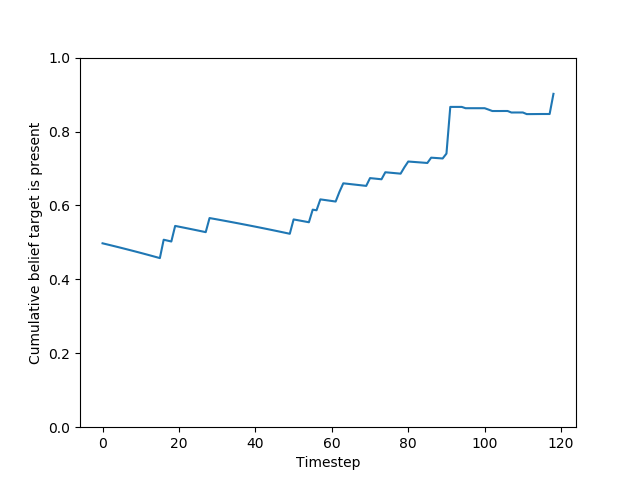
\includegraphics[width=6cm]{Chapters/MultiAgentTargetDetection/Figs/Results/BeliefEvolution/MiscalibratedSensor/05-02/SweepBeliefEvolution4.png}}}%
    \qquad
    \subfloat[Sample run using Saccadic search strategy]{{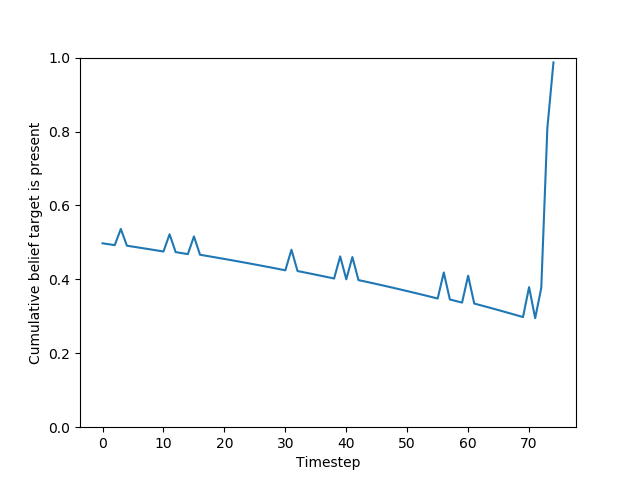
\includegraphics[width=6cm]{Chapters/MultiAgentTargetDetection/Figs/Results/BeliefEvolution/MiscalibratedSensor/05-02/SaccadicBeliefEvolution4.png} }}%
    \caption{Sample runs with miscalibrated sensor model parameters fpr=0.05, fnr=0.02}%
    \label{fig:MiscalibratedSensorFPR005}%
\end{figure}

\begin{figure}
\centering
    \subfloat[Sample run using Random search strategy]{{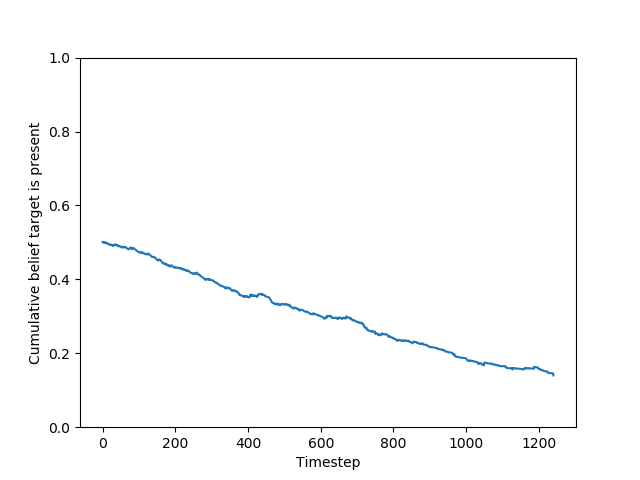
\includegraphics[width=6cm]{Chapters/MultiAgentTargetDetection/Figs/Results/BeliefEvolution/MiscalibratedSensor/4-4/RandomBeliefEvolution2.png}}}%
    \qquad
    \subfloat[Sample run using Saccadic search strategy]{{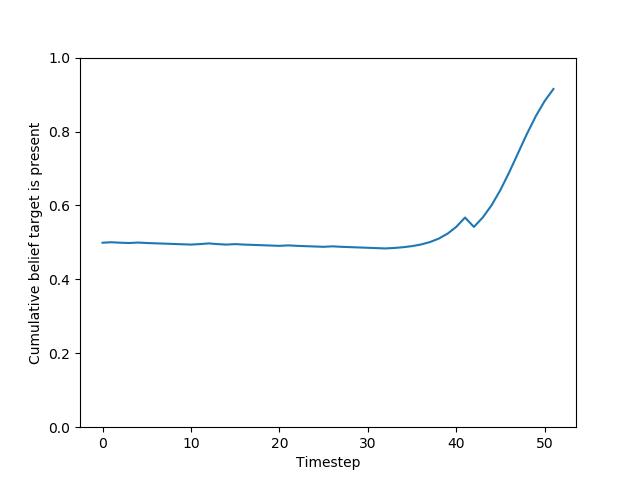
\includegraphics[width=6cm]{Chapters/MultiAgentTargetDetection/Figs/Results/BeliefEvolution/MiscalibratedSensor/4-4/SaccadicBeliefEvolution0.png} }}%
    \caption{Sample runs with miscalibrated sensor model parameters fpr=0.4, fnr=0.4}%
    \label{fig:MiscalibratedSensorFPR04}%
\end{figure}

Table \ref{table:MiscalibratedSensor} displays the results of running a simulation with a single agent and a single target while varying the parameters of the sensor model. The sensor model is parameterised using a false positive rate and false negative rate, detailed in equation \ref{eqn:EvidenceVarsProbs}. We deliberately chose extreme values for these parameters to show the effects of an extreme miscalibration, which can be thought of as a worst case scenario. We discuss the results in terms of underestimating and overestimating the true sensor parameters:
\begin{enumerate}
    \item When the model is calibrated to underestimate the rate at which the sensor will detect false negatives and false positives (the rows which have a sensor model fpr = 0.05, sensor model fnr = 0.02 in Table \ref{table:MiscalibratedSensor}), relative to the correctly calibrated sensor model (the rows which have a sensor model fpr = 0.2, sensor model fnr = 0.15 in Table \ref{table:MiscalibratedSensor}), both positive and negative observations will have a greater effect on the change in the shape of the distribution of the agent's belief, since the sensor model is more confident that the readings are correct. This means that is easier to cross the decision threshold of the SPRT due to spurious observations. For example, it would require 3, 5 and 17 positive consecutive observations at the same location to cross the upper SPRT threshold in the cases that the sensor model is calibrated with fpr=0.05/fnr=0.02, fpr=0.2/fnr=0.15, fpr=0.4/fnr=0.4 respectively.
    Underestimating the true sensor parameters leads to a much higher incorrect localisation rate in the adaptive search strategies in relation to the non-adaptive search strategies, which is evident in the Proportion Incorrectly Localised column of Table \ref{table:MiscalibratedSensor}. The reason for this is that the non-adaptive search strategies do not follow up on positive observations. The agent belief increases a relatively large amount with every positive observation, which actually arrive at a much higher rate (0.2066) than the sensor is calibrated for (0.0593). For example, if the agent immediately makes a positive observation, its belief will jump from 0.5 to 0.5425. Figure \ref{fig:MiscalibratedSensorFPR005} (a) shows the evolution of the agent's cumulative belief that the target is present in the search region. Relatively large jumps in cumulative belief due to the miscalibrated sensor model are clearly visible. This is in contrast with the adaptive strategies, where the agent re-samples positive observations, which drives the agent's belief back down in the case of spurious positives, which is visible in Figure \ref{fig:MiscalibratedSensorFPR005} (b).
    
    %\textit{Proportion Incorrectly Localised} column of table \ref{table:MiscalibratedSensor}. Similarly, we see that the false negative rate increases, as the miscalibrated model causes the belief in the target being absent for the region to increase more sharply with negative observations than the correctly calibrated sensor model. The mean time to decision (TTD) increases in this case because the belief in the target presence jumps disproportionately when a positive observation is made relative to a negative observation. The ratio of the sensor model FPR to FNR is approximately half the true ratio, which means the effect of positive observations is underestimated, causing the agent to delay the conclusion in a positive target localisation.
    \item Conversely, when the model is calibrated to overestimate the rate at which the sensor will record false positives and false negatives (the rows which have a sensor model fpr = 0.4, sensor model fnr = 0.4 in Table \ref{table:MiscalibratedSensor}), the belief distribution changes much more gradually given positive or negative observations. This means that crossing the decision thresholds given by the SPRT will require many more positive or negative readings, which leads to much higher mean times to decision (TTD) for all search strategies. As a lower bound, the SPRT would require 447 consecutive negative observations when running the sweep search in order to conclude that the target is not present. In the adaptive cases, once a positive observation is made at a given location, the agent's belief usually becomes highest at that location, which causes the agent to sample there again. Once it visits the true target location, usually it will receive a sufficient number of positive observations to keep sampling it, which causes its cumulative belief to steadily increase, as shown in Figure \ref{fig:MiscalibratedSensorFPR04} (a). The non-adaptive methods do not exhibit this behaviour since they are unbiased sampling methods. They do not re-sample when they come across a positive observation, which causes their cumulative belief in the target presence to gradually drop. If they do not experience consecutive positive observations when they visit the true target location, usually their belief will drop below the SPRT threshold, as can be seen in Figure \ref{fig:MiscalibratedSensorFPR04} (b).
\end{enumerate}
\break

\subsubsection{Varying the number of targets present in the region}\label{subsubsec:VaryingNoTargets}
\begin{landscape}
\centering
\vspace*{\fill}
\begin{table}[h!]
    \centering
    \begin{tabular}{| >{\centering} m{18mm} | >{\centering}m{20mm} | >{\centering}m{18mm} | >{\centering}m{20mm} | >{\centering}m{20mm} | >{\centering}m{20mm} | m{60mm} <{\centering}|}
    \hline
       Strategy & Number of Targets Present & E[Time To Decision] & SD[Time To Decision] & False Negative Rate & Proportion Incorrect Localised & Decision Matrix\\
        \hline
        $\epsilon$ -Greedy & 1 & 112.93 & 62.38 & 0.152 & 0.040 & ToDo\\
        $\epsilon$ -Greedy & 2 & 155.77 & 50.93 & ToDo & ToDo & \begin{tabular}{l|l|c|c|c}
\multicolumn{2}{c}{}&\multicolumn{2}{c}{diagnosis}&\\
\cline{3-4}
\multicolumn{2}{c|}{}&0&1&\multicolumn{1}{c}{Total}\\
\cline{2-4}
\multirow{2}{*}{G}& 0 & $a$ & $b$ & $a+b$\\
\cline{2-4}
& 1 & $c$ & $d$ & $c+d$\\
\cline{2-4}
\multicolumn{1}{c}{} & \multicolumn{1}{c}{Total} & \multicolumn{1}{c}{$a+c$} & \multicolumn{    1}{c}{$b+d$} & \multicolumn{1}{c}{$N$}\\
\end{tabular} \\
        $\epsilon$ -Greedy & 3 & 175.84 & 42.78 & ToDo & ToDo & \begin{tabular}{l|l|c|c|c|}
\multicolumn{2}{c}{}&\multicolumn{2}{c}{\#Correct G}&\\
\cline{3-5}
\multicolumn{2}{c|}{}&0&1&2%\multicolumn{1}{c}{Total}
\\
\cline{2-5}
\multirow{2}{*}{\# G}& 0 & $a$ & $b$ & $c$\\
\cline{2-5}
& 1 & $e$ & $f$ & $g$\\
\cline{2-5}
& 2 & $h$ & $i$ & $j$\\
\cline{2-5}
\multicolumn{1}{c}{} & \multicolumn{1}{c}{Total} & \multicolumn{1}{c}{$x$} & \multicolumn{    1}{c}{$y$} & \multicolumn{1}{c}{$N$}\\
\end{tabular} \\
        \hline
        Sweep & 1 & 601.57 & 183.45 & 0.1254 & 0.0454  & ToDo\\
        Sweep & 2 & 708.02 & 206.57 & ToDo & ToDo  & ToDo\\
        Sweep & 3 & 770.00 & 223.96 & ToDo & ToDo & ToDo \\
        \hline
        Saccadic & 1 & 98.83 & 56.13 & 0.1588 & 0.037 & ToDo \\
        Saccadic & 2 & 135.64 & 45.43 & ToDo & ToDo & ToDo \\
        Saccadic & 3 & 154.59 & 36.62 & ToDo & ToDo & ToDo \\
        \hline
        Random & 1 & 629.55 & 282.95 & 0.1368 & 0.0336 & ToDo \\
        Random & 2 & 787.44 & 287.61 & ToDo & ToDo & ToDo \\
        Random & 3 & 882.74 & 295.05 & ToDo & ToDo & ToDo \\
        \hline
    \end{tabular}
    \caption{Results of running the target localisation simulation with a \textbf{varying number of targets}. Fixed P(T1) = 0.1, p(T2) = 0.15, Simulated Sensor FPR = 0.2, Simulated Sensor FNR = 0.15, Sensor Model FPR = 0.2, Sensor Model FNR = 0.15, }
    \label{table:PriorUniform}
\end{table}
\end{landscape}

\break

\begin{table}[h!]
    \centering
    \begin{tabular}{| >{\centering} m{17mm} | >{\centering}m{13mm} | >{\centering}m{14mm} | >{\centering}m{15mm} | m{72mm} <{\centering}|}
    \hline
       Strategy & \# Targets Present & E[TTD] & SD [TTD] & Decision Matrix Showing \# Returned Target Locations (Rows) vs. \# Targets Correctly Localised (Cols).\\
        \hline
        $\epsilon$ -Greedy & 1 & 112.93 & 62.38 & {
        \centering
        \begin{tabular}{c|c|c|}
           \multicolumn{1}{c}{} & \multicolumn{2}{c}{ } \\
           \multicolumn{1}{c}{} & \multicolumn{1}{c}{0}  & \multicolumn{1}{c}{1} \\
           \cline{2-3}
            0 & 0.152 & 0 \\ \cline{2-3}
            1 & 0.0400 & 0.8080 \\\cline{2-3}
            \multicolumn{3}{c}{}
        \end{tabular}
        }\\
        $\epsilon$ -Greedy & 2 & 155.77 & 50.93 & 
        {
        \centering
        \begin{tabular}{c|c|c|c|}
           \multicolumn{1}{c}{} & \multicolumn{3}{c}{ } \\
           \multicolumn{1}{c}{} & \multicolumn{1}{c}{0}  & \multicolumn{1}{c}{1}  & \multicolumn{1}{c}{2} \\
           \cline{2-4}
            0 & 0.0218 & 0 & 0 \\ \cline{2-4}
            1 & 0.0012 & 0.2644 & 0 \\\cline{2-4}
            2 & 0.0006 & 0.0474 & 0.6646 \\\cline{2-4}
        \end{tabular}
        }
        \\
        $\epsilon$ -Greedy & 3 & 175.84 & 42.78 &
        {
        \centering
        \begin{tabular}{c|c|c|c|c|}
           \multicolumn{1}{c}{} & \multicolumn{4}{c}{ } \\
           \multicolumn{1}{c}{} & \multicolumn{1}{c}{0}  & \multicolumn{1}{c}{1}  & \multicolumn{1}{c}{2}& \multicolumn{1}{c}{3} \\
           \cline{2-5}
            0 & 0.0038 & 0 & 0 & 0\\ \cline{2-5}
            1 & 0 & 0.0596 & 0 & 0 \\\cline{2-5}
            2 & 0 & 0.0064 & 0.3170 & 0\\\cline{2-5}
            3 & 0 & 0.0002 & 0.0510 & 0.5620\\\cline{2-5}
            \multicolumn{4}{c}{}\\
        \end{tabular}
        }
        \\
        \hline
        Sweep & 1 & 601.57 & 183.45 & {
        \centering
        \begin{tabular}{c|c|c|}
           \multicolumn{1}{c}{} & \multicolumn{2}{c}{ } \\
           \multicolumn{1}{c}{} & \multicolumn{1}{c}{0}  & \multicolumn{1}{c}{1} \\
           \cline{2-3}
            0 & 0.1254 & 0 \\ \cline{2-3}
            1 & 0.0454 & 0.8292 \\\cline{2-3}
            \multicolumn{3}{c}{}
        \end{tabular}
        }\\
        Sweep & 2 & 708.02 & 206.57 &
        {
        \centering
        \begin{tabular}{c|c|c|c|}
           \multicolumn{1}{c}{} & \multicolumn{3}{c}{ } \\
           \multicolumn{1}{c}{} & \multicolumn{1}{c}{0}  & \multicolumn{1}{c}{1}  & \multicolumn{1}{c}{2} \\
           \cline{2-4}
            0 & 0.0106 & 0 & 0 \\ \cline{2-4}
            1 & 0.0002 & 0.181 & 0 \\\cline{2-4}
            2 & 0.0018 & 0.0666 & 0.7398 \\\cline{2-4}
        \end{tabular}
        }
        \\
        Sweep & 3 & 770.00 & 223.96 & 
        {
        \centering
        \begin{tabular}{c|c|c|c|c|}
           \multicolumn{1}{c}{} & \multicolumn{4}{c}{ } \\
           \multicolumn{1}{c}{} & \multicolumn{1}{c}{0}  & \multicolumn{1}{c}{1}  & \multicolumn{1}{c}{2}& \multicolumn{1}{c}{3} \\
           \cline{2-5}
            0 & 0.002 & 0 & 0 & 0\\ \cline{2-5}
            1 & 0.0002 & 0.022 & 0 & 0 \\\cline{2-5}
            2 & 0 & 0.0014 & 0.2104 & 0\\\cline{2-5}
            3 & 0.0002 & 0.0034 & 0.082 & 0.6784\\\cline{2-5}
            \multicolumn{4}{c}{}
        \end{tabular}
        }
        \\
        \hline
        \end{tabular}
        \caption{Results of running the target localisation simulation with 1,2 and 3 targets for sweep search and $\epsilon$-greedy search.}
        \label{table:MultipleTargetEGSweep}
        \end{table}
        
        
        
        
        
        \begin{table}[h!]
        \begin{tabular}{| >{\centering} m{17mm} | >{\centering}m{13mm} | >{\centering}m{14mm} | >{\centering}m{15mm} | m{72mm} <{\centering}|}
        \hline
        Strategy & No. Targets Present & E[TTD] & SD [TTD] & Decision Matrix Showing \# Returned Target Locations (Rows) vs. \# Targets Correctly Localised (Cols).\\
        \hline
        Saccadic & 1 & 98.83 & 56.13 & {
        \centering
        \begin{tabular}{c|c|c|}
           \multicolumn{1}{c}{} & \multicolumn{2}{c}{ } \\
           \multicolumn{1}{c}{} & \multicolumn{1}{c}{0}  & \multicolumn{1}{c}{1} \\
           \cline{2-3}
            0 & 0.1588 & 0 \\ \cline{2-3}
            1 & 0.0370 & 0.8042 \\\cline{2-3}
            \multicolumn{3}{c}{}
        \end{tabular}
        } \\
        Saccadic & 2 & 135.64 & 45.43 & 
        {
        \centering
        \begin{tabular}{c|c|c|c|}
           \multicolumn{1}{c}{} & \multicolumn{3}{c}{ } \\
           \multicolumn{1}{c}{} & \multicolumn{1}{c}{0}  & \multicolumn{1}{c}{1}  & \multicolumn{1}{c}{2} \\
           \cline{2-4}
            0 & 0.0258 & 0 & 0 \\ \cline{2-4}
            1 & 0.0014 & 0.2664 & 0 \\\cline{2-4}
            2 & 0 & 0.0448 & 0.6616 \\\cline{2-4}
        \end{tabular}
        }
        \\
        Saccadic & 3 & 154.59 & 36.62 &
        {
        \centering
        \begin{tabular}{c|c|c|c|c|}
           \multicolumn{1}{c}{} & \multicolumn{4}{c}{ } \\
           \multicolumn{1}{c}{} & \multicolumn{1}{c}{0}  & \multicolumn{1}{c}{1}  & \multicolumn{1}{c}{2}& \multicolumn{1}{c}{3} \\
           \cline{2-5}
            0 & 0.0052 & 0 & 0 & 0\\ \cline{2-5}
            1 & 0.0002 & 0.07 & 0 & 0 \\\cline{2-5}
            2 & 0 & 0.0036 & 0.3246 & 0\\\cline{2-5}
            3 & 0 & 0.0006 & 0.0458 & 0.55\\\cline{2-5}
            \multicolumn{4}{c}{}
        \end{tabular}
        }
        \\
        \hline
        Random & 1 & 629.55 & 282.95 & {
        \centering
        \begin{tabular}{c|c|c|}
           \multicolumn{1}{c}{} & \multicolumn{2}{c}{ } \\
           \multicolumn{1}{c}{} & \multicolumn{1}{c}{0}  & \multicolumn{1}{c}{1} \\
           \cline{2-3}
            0 & 0.1368 & 0 \\ \cline{2-3}
            1 & 0.0336 & 0.8296 \\\cline{2-3}
            \multicolumn{3}{c}{}
        \end{tabular}
        } \\
        Random & 2 & 787.44 & 287.61 & 
        {
        \centering
        \begin{tabular}{c|c|c|c|}
           \multicolumn{1}{c}{} & \multicolumn{3}{c}{ } \\
           \multicolumn{1}{c}{} & \multicolumn{1}{c}{0}  & \multicolumn{1}{c}{1}  & \multicolumn{1}{c}{2} \\
           \cline{2-4}
            0 & 0.0166 & 0 & 0 \\ \cline{2-4}
            1 & 0.0012 & 0.1872 & 0 \\\cline{2-4}
            2 & 0.0004 & 0.053 & 0.7416 \\\cline{2-4}
        \end{tabular}
        }
        \\
        Random & 3 & 882.74 & 295.05 & 
        {
        \centering
        \begin{tabular}{c|c|c|c|c|}
           \multicolumn{1}{c}{} & \multicolumn{4}{c}{ } \\
           \multicolumn{1}{c}{} & \multicolumn{1}{c}{0}  & \multicolumn{1}{c}{1}  & \multicolumn{1}{c}{2}& \multicolumn{1}{c}{3} \\
           \cline{2-5}
            0 & 0.0014 & 0 & 0 & 0\\ \cline{2-5}
            1 & 0.0002 & 0.0248 & 0 & 0 \\\cline{2-5}
            2 & 0 & 0.0014 & 0.2138 & 0\\\cline{2-5}
            3 & 0 & 0.0022 & 0.0608 & 0.6954 \\\cline{2-5}
            \multicolumn{4}{c}{}
        \end{tabular}
        }
        \\
        \hline
    \end{tabular}
    \caption{Results of running the target localisation simulation with 1,2 and 3 targets for saccadic search and random search.}
    \label{table:MultipleTargetSaccadicRandom}
\end{table}

Tables \ref{table:MultipleTargetEGSweep} and \ref{table:MultipleTargetSaccadicRandom} display the results of running a simulation with a single agent with a varying number of targets in the search region. We ran algorithm \ref{alg:MultiTargetLocalisation} to carry out the localisation procedure. The results show that the mean time to decision increases sub-linearly with respect to the number of targets present. The rows of the decision matrix show the proportions of how many target locations are returned by the agent and the columns show how many targets are correctly localised. The results indicate that the more targets that are present, the less willing the agent is to conclude that the are no targets present, but that it is also less willing to conclude that the maximum number of targets are present. The reason why the agent consistently returns 0 target locations at a lower rate when there is more targets present can be explained by the miscalibrated sensor results; since there are more targets present, the number of observed true positives is greater than the calibrated values. This essentially means that the sensor model fnr is over-estimated, which leads to a much lower search false negative rate. This could be overcome by calibrating the sensor model with the fnr and fpr that would arise from the number of targets suspected to be present in the region, and re-calibrating it each time a target is localised by the agent.
\break


\subsection{Varying number of search agents}

This experiment explored how varying the number of agents involved in the search impacted on the effectiveness of the search. We assumed that agents communicated their most recent observation to all other agent at each time step, which the other agents used to update their local belief that the target it present in the region.


\begin{table}[H]
    \centering
    \begin{tabular}{| >{\centering} m{18mm} | >{\centering}m{20mm} | >{\centering}m{18mm} | >{\centering}m{20mm} | >{\centering}m{20mm} | m{20mm} <{\centering}|}
    \hline
       Strategy & \# Agents & Mean TTD & Sample SD[TTD] & False Negative Rate & Proportion Incorrectly Localised \\
        \hline
        $\epsilon$-Greedy & 1 & 112.9258 & 62.3798 & 0.1516 & 0.0398 \\
        $\epsilon$-Greedy & 2 & 65.5912 & 34.3248 & 0.1568 & 0.0314 \\
        $\epsilon$-Greedy & 3 & 47.5176 & 24.9861 & 0.1428 & 0.0262 \\
        \hline
        Sweep & 1 & 601.5697 & 183.4529 & 0.1254 & 0.0454 \\
        Sweep & 2  & 303.7328 & 94.2748 & 0.1232 & 0.0466 \\
        Sweep & 3 & 204.8172 & 65.1273 & 0.1252 & 0.0408 \\
        \hline
        Saccadic & 1 & 98.8274 & 56.1298 & 0.1588 & 0.0370 \\
        Saccadic & 2 & 75.3466 & 39.9718 & 0.1520 & 0.0132 \\
        Saccadic & 3 & 65.0774 & 33.9798 & 0.1598 & 0.0090 \\
        \hline
        Random & 1 & 629.5462 & 282.9514 & 0.1368 & 0.0366 \\
        Random & 2 & 315.0082 & 140.3954 & 0.1254 & 0.0366  \\
        Random & 3 & 211.4242 & 94.7801 & 0.1222 & 0.0448\\
        \hline
    \end{tabular}
   \caption{Results of running the target localisation simulation with a varying number of homogeneous agents for each implemented search strategy.}
    \label{table:VaryingNumberOfAgents}
\end{table}

Table \ref{table:VaryingNumberOfAgents} shows the results of running the search with 1, 2 and 3 homogeneous agents. Each agent is initialised with the same parameters, but start at independently chosen random locations. They receive new observations from other agents at each time-step and then record their own observation. We did not assume that there could be corrupted/interrupted transmissions, although this could be investigated in future work.
%The results agree closely with \cite{Chung2008Multi-agentFramework}. 
Figure 2 and Figure 3 of \cite{Chung2008Multi-agentFramework} show sample runs of adaptive and non-adaptive search strategies for the same simulation configuration. The observed results matched our expectations based on \cite{Chung2008Multi-agentFramework}, where the largest relative reduction in the mean TTD is found in the non-adaptive cases. This is because the non-adaptive cases use unbiased sampling methods. The sweep search method samples all grid cells an equal number of times, so running multiple agents is equivalent to running a single agent with the non-adaptive strategy that can sample multiple times on each time-step rather than just once. This implies the search time is inversely proportional to the number of agents used in the non-adaptive cases, supported by Table \ref{table:VaryingPriorDistribution}. Since the agents first record a sensor observation and update their belief before updating their belief based on other agent observations made at the current time-step, sometimes an agent will end its search before the other agents, which means that the effect of having multiple agents is lessened. This is more prevalent when using the adaptive strategies since when the agents locate the source correctly, there is a chance that one could receive a false negative, while the others terminate with true positive observations. This leads the last agent to make extra observations, inflating the mean TTD. The unbiased methods do not exhibit this behaviour as much and usually terminate when one agent at the target location makes a positive observation which is shared among other agents who are not at the target location and who then also subsequently terminate.


\label{sec:SimulationResults}

\section{Conclusion and Future Work}
%\note{From C\&B: In contrast with these previous works, the pre-sented research herein offers a sequential Bayesian formulation that addresses joint dependence of probabilities, the presence of both false-negative and false-positive detections, and constraints on searcher motion}

%\note{however,  such  costly near-optimal approaches may be less desirable than algorithms that provide “good enough” solutions, where the application re-quires computationally limited platforms, such as educational robots  or  miniaturized  embedded  system}

This chapter described a system which was designed to solve the problem of \textit{target localisation} using RAVs. Our system was designed on the basis of previous work, outlined in Section \ref{sec:StochasticTargetLocalisationRelatedLiterature}. The system's performance was analysed using Monte Carlo simulation and we explored the trade-off between minimising Time-To-Decision (TTD) against drawing incorrect conclusions. The results largely matched what we expected to see, but they offer a solid basis on which to set system parameters in order to achieve a desired level of performance. We evaluated four search strategies. Two were adaptive, $\epsilon$-greedy search and Saccadic search, meaning they sampled the search region in a biased manner in the hope of converging quickly on the target location. Two were unbiased, Sweep search and Random search, which offered a baseline for comparison and facilitated analysis which was useful in showing how the system reacts to perturbations in the values of the parameters.

We first found that the shape of the initial belief distribution has a large bearing on the time-to-decision, where the use of an uninformed initial belief distribution causes a large increase in the search time relative to the use of an initial belief distribution that is aligned with the shape of the true distribution. The effect was greatest while using the adaptive search methods, which offered respective reductions in mean time to decision of 80.1\% and 85.3\% for the $\epsilon$-greedy search and Saccadic search strategies. The results also showed that the rate at which the system incorrectly concluded that the target was not present also dropped significantly, with respective reduction in mean time to decision of 80.1\% and 75.6.3\% for the $\epsilon$-greedy search and Saccadic search strategies. \par

When the initial cumulative belief that the target was present for a uniform distribution was set to 0.25, we observed a drop in the mean time to decision for all search strategies. The adaptive strategies followed resampled the locations of false positives, which quickly drove the cumulative belief below the lower SPRT threshold prematurely. The non-adaptive strategies also experienced enough negative observations in relation to positives to terminate prematurely. This led to an inflated rate at which the system concluded the source was not present. In the case where the initial cumulative belief that the target was present started at 0.75, the adaptive methods saw a slight increase in the mean time to decision relative to the case where the initial cumulative belief was set to 0.5. The evidence suggested that since a comparable number of consecutive positive observations at the true target location would push the agent's belief over the SPRT upper threshold, the relatively high number of samples needed to make a negative conclusion was the cause. The non-adaptive methods saw a decrease in the mean time to decision because the initial belief started closer to the boundary and required  fewer positive observations to cross the upper SPRT threshold.\par


When we set the sensor model parameters to under-estimate the actual false positive and false negative rates of observations, the results we observed matched our expectations. Since the model was more confident about observations, the agent's belief fluctuated more aggressively, which made it easier to cross the upper and lower decision thresholds. This led to a drop in the mean time to decision for all search strategies relative the case with the correctly calibrated sensor (40.4\%, 37.4\%, 71.4\%, 78.0\% for $\epsilon$-greedy, Saccadic, Random and Sweep respectively). Conversely, when the sensor model parameters over-estimated the fpr and fnr of observations, the agent's belief fluctuated in a much more gentle manner, which meant it took many more observations to reach the threshold set by the SPRT compared to with the case with the correctly calibrated sensor (75.0\%, 43.9\%, 233.7\%, 255.5\% for $\epsilon$-greedy, Saccadic, Random and Sweep respectively). When the sensor model parameters were under-estimated, the proportion of simulation runs where the target was incorrectly localised shot up, since the relative true positive rate was lower than in the case where the sensor model fpr and fnr were set to 0.2 and 0.15 respectively.\par

Multiple targets caused the mean time to decision to increase sub-linearly with the number of targets present for all search strategies. This is because the agent ran a sequential procedure, which meant information gathered while localising the first target could be used to expedite the localisation of subsequent targets. The presence of two targets instead of one increased the mean time to decision by 37.9\%, 17.7\%, 37.3\%, 25.1\% for $\epsilon$-greedy, Sweep, Saccadic and Random respectively. The presence of three targets instead of one increased the mean time to decision by 55.7\%,  28.0\%, 56.4\%, 40.2\% for $\epsilon$-greedy, Sweep, Saccadic and Random respectively. These represent marked improvements over the naive case, where re-starting the search once a target had been localised with the same initial belief distribution would have double and tripled the mean time to decision for two and three targets. The results show that as more targets were introduced to the target region, the more likely the search procedure was to terminate prematurely, concluding that there were fewer targets present than there actually were. Addressing this could be part of future work.\par

The use of multiple agents cut the mean time to decision for each of the search strategies while maintaining the rates at which an incorrect conclusion was drawn. The use of two agents cut the mean time to decision by 42.0\%, 50.0\%, 23.4\%, 50.0\% for $\epsilon$-greedy, Sweep, Saccadic and Random respectively. The use of three agents cut the mean time to decision by 58.0\%, 66.0\%, 34.2\%, 66.4\% for $\epsilon$-greedy, Sweep, Saccadic and Random respectively. We anticipate that introducing a maximum radius in which the agents can communicate with each other, with the probability of communicating successfully inversely proportional to the distance between agents, would mean adding extra agents would have less of an effect on the mean time to decision but would help to stabilise the rates at which the system mistakenly concludes the search.

\subsection{Future Work}
Future work for the problem of target localisation has been outlined in \cite{Chung2007ASearch}, \cite{Chung2008Multi-agentFramework}, \cite{Chung2012AnalysisStrategies}, \cite{Kriheli2016OptimalInspections}. We summarise the previously identified future work, along with our own suggestions, as follows:

\begin{enumerate}

    \item We did not take into account battery limitations for the RAV agents. In reality, they would need to periodically recharge while carrying out the search, as mentioned in section \ref{sec:SceneSurveyingBatteryConstraints} of chapter \ref{chapter:SceneSurveying}. We hypothesise that a battery model could be learned using the Expectation-Maximisation (E-M) algorithm \cite{Dempster1977MaximumAlgorithm}. This could then be integrated with the search strategy to prevent the RAVs from running out of power while searching.
    \item In this work, all simulations were ran with a target present. Future work could investigate system performance with the absence of a target, or with the presence of false targets that could be considered as an adversarial measure taken to fool the system.
    \item We assumed that agents could localise \textit{themselves} accurately, which is not always the case. Research into how agents can perform the search without a deterministic location sensor could incorporate this extra level of uncertainty.
    \item Our simulation involving multiple agents assumed that they are homogeneous. Future work could explore the use of heterogeneous agents in carrying out the target localisation task. This could involve using agents with different sensing capabilities, different operational speeds, different battery lives and different search strategies. Future work could also investigate how to optimise various configurations to provide a more robust and efficient system, building on \cite{Chung2008Multi-agentFramework}.
    \item The performance measure discussed in Section \ref{sssection:PerfMeas} only takes into account the time taken to localise the target. It could be modified to take into account other factors such as energy expended by the agents. This may allow for a more realistic trade-off than solely focusing on making the correct decision in the least possible amount of time.
    \item It is becoming more common for RAVs to integrate a multitude of sensors in their platforms. For example, in the ROCSAFE project \cite{Bagherzadeh2017ROCSAFE:Incidents}, advanced lightweight senors are being developed to be used with a RAV to remotely detect potentially hazardous substances. Multi-sensor fusion techniques have been shown in certain cases to be highly effective in identifying outliers and creating more robust estimators of true environment state. The review paper \cite{Khaleghi2013MultisensorState-of-the-art} discusses challenges and promising future areas related to research involving the fusion of data from multiple sensors. Exploring the improvements that a multi-sensor approach could potentially provide could be a future avenue of research.
    \item  We followed the approach of \cite{Chung2007ASearch} in developing a sensor model. The approach is very general, but is highly susceptible to providing poor results due to miscalibration, evident in Table \ref{table:MiscalibratedSensor}. Developing a more advanced sensor model that is specific to common tasks, such as object detection, may yield a more robust and efficient system. For example, \cite{Symington2010ProbabilisticUAVs} outlines a sensor model which was calibrated with varying heights of the RAV and \cite{Thrun:2005:ProbabilisticRobotics} outlines sensor models commonly used with robotic vehicles.
    \item Running the system in a realistic setting would offer insight in the practicality of the system. For example, we ran the agent software on a desktop machine, but in reality it would likely be running on an embedded system with a reduced computational ability relative to a desktop. This may show the system is infeasible due to constraints such as memory size or processor speed. Future research could involve running the system on realistic hardware to evaluate its feasibility. In the future, we intend to run the system using the high-fidelity simulation discussed in Chapter \ref{chap:HighFidelitySim}, with the agent software running on raspberry pi devices. This will give a stronger indication of how the system may potentially perform in the real world.
    \item Further theoretical analysis of the system could offer insight into how it could be improved. In \cite{Chung2012AnalysisStrategies} and \cite{Chung2009ProbabilisticAgents}, special cases are analysed in order to elicit properties, such as the rate of change of agent belief, which can be useful in devising strategies to improve the search performance.
\end{enumerate}